\documentclass[twocolumn]{article}
%\usepackage[left=0.7in,right=0.7in,top=1in,bottom=1in]{geometry}
\setlength{\columnsep}{2\columnsep}
\usepackage[utf8]{inputenc}
\usepackage{amssymb}
\usepackage{amsmath}
\usepackage[longend,linesnumbered,ruled]{algorithm2e}
\usepackage{graphicx}
\usepackage{siunitx}
\usepackage[round,authoryear,sort]{natbib}
\usepackage{url}
\usepackage[pdftex,colorlinks=true]{hyperref}
\usepackage{fancyhdr}
\usepackage{multirow}
\usepackage{booktabs}
\usepackage{setspace}

% Define style for urls
\urlstyle{same}

% Define special units
\DeclareSIUnit\mgal{\milli Gal}

% Define inverse symbol with shorter minus
\newcommand{\inv}{^{\text{-}1}}
\newcommand{\trans}{^{\text{T}}}

% Import files with parameter values generated by notebooks
\newcommand{\Gal}{Gal}
\newcommand{\NPrisms}{64}
\newcommand{\ModelEasting}{111319~m}
\newcommand{\ModelNorthing}{111319~m}
\newcommand{\ModelDepth}{10000~m}
\newcommand{\ModelMinDensity}{-900~kg~m$^{-3}$}
\newcommand{\ModelMaxDensity}{500~kg~m$^{-3}$}
\newcommand{\SurveyEasting}{111319~m}
\newcommand{\SurveyNorthing}{110576~m}
\newcommand{\SurveyNoise}{1~mGal}
\newcommand{\GroundSurveyPoints}{963}
\newcommand{\GroundSurveyMinHeight}{0~m}
\newcommand{\GroundSurveyMaxHeight}{2052.2~m}
\newcommand{\AirborneSurveyPoints}{5673}
\newcommand{\AirborneSurveyMinHeight}{359~m}
\newcommand{\AirborneSurveyMaxHeight}{1255~m}
\newcommand{\TargetHeight}{2000~m}
\newcommand{\TargetSpacing}{2~m}
\newcommand{\TargetEastingSize}{57}
\newcommand{\TargetNorthingSize}{56}
\newcommand{\GroundSourceBelowDataConstantDepthDamping}{\num{e-4}, \num{e-3},$\dots$, \num{e2}}
\newcommand{\GroundSourceBelowDataConstantDepthDepth}{\numrange{1000}{17000}, step size \num{2000}}
\newcommand{\GroundSourceBelowDataRelativeDepthDamping}{\num{e-4}, \num{e-3},$\dots$, \num{e2}}
\newcommand{\GroundSourceBelowDataRelativeDepthDepth}{\numrange{1000}{17000}, step size \num{2000}}
\newcommand{\GroundSourceBelowDataVariableDepthDamping}{\num{e-4}, \num{e-3},$\dots$, \num{e2}}
\newcommand{\GroundSourceBelowDataVariableDepthDepthFactor}{\numlist{0.1;0.5;1;2;3;4;5;6}}
\newcommand{\GroundSourceBelowDataVariableDepthDepth}{\numrange{0}{1400}, step size \num{200}}
\newcommand{\GroundSourceBelowDataVariableDepthKNearest}{\numlist{1;5;10;15}}
\newcommand{\GroundBlockAveragedSourcesConstantDepthDamping}{\num{e-4}, \num{e-3},$\dots$, \num{e2}}
\newcommand{\GroundBlockAveragedSourcesConstantDepthDepth}{\numrange{1000}{17000}, step size \num{2000}}
\newcommand{\GroundBlockAveragedSourcesConstantDepthSpacing}{\numlist{1000;2000;3000;4000}}
\newcommand{\GroundBlockAveragedSourcesRelativeDepthDamping}{\num{e-4}, \num{e-3},$\dots$, \num{e2}}
\newcommand{\GroundBlockAveragedSourcesRelativeDepthDepth}{\numrange{1000}{17000}, step size \num{2000}}
\newcommand{\GroundBlockAveragedSourcesRelativeDepthSpacing}{\numlist{1000;2000;3000;4000}}
\newcommand{\GroundBlockAveragedSourcesVariableDepthDamping}{\num{e-4}, \num{e-3},$\dots$, \num{e2}}
\newcommand{\GroundBlockAveragedSourcesVariableDepthSpacing}{\numlist{1000;2000;3000;4000}}
\newcommand{\GroundBlockAveragedSourcesVariableDepthDepthFactor}{\numlist{0.1;0.5;1;2;3;4;5;6}}
\newcommand{\GroundBlockAveragedSourcesVariableDepthDepth}{\numrange{0}{1400}, step size \num{200}}
\newcommand{\GroundBlockAveragedSourcesVariableDepthKNearest}{\numlist{1;5;10;15}}
\newcommand{\GroundGridSourcesConstantDepthDamping}{\numlist{e1;e2;e3;e4}}
\newcommand{\GroundGridSourcesConstantDepthDepth}{\numrange{1000}{9000}, step size \num{2000}}
\newcommand{\GroundGridSourcesConstantDepthSpacing}{\numlist{1000;2000;3000;4000}}
\newcommand{\AirborneSourceBelowDataConstantDepthDamping}{\num{e-4}, \num{e-3},$\dots$, \num{e2}}
\newcommand{\AirborneSourceBelowDataConstantDepthDepth}{\numrange{1000}{17000}, step size \num{2000}}
\newcommand{\AirborneSourceBelowDataRelativeDepthDamping}{\num{e-4}, \num{e-3},$\dots$, \num{e2}}
\newcommand{\AirborneSourceBelowDataRelativeDepthDepth}{\numrange{1000}{17000}, step size \num{2000}}
\newcommand{\AirborneSourceBelowDataVariableDepthDamping}{\num{e-4}, \num{e-3},$\dots$, \num{e2}}
\newcommand{\AirborneSourceBelowDataVariableDepthDepthFactor}{\numrange{1}{6}, step size \num{1}}
\newcommand{\AirborneSourceBelowDataVariableDepthDepth}{\numrange{50}{1450}, step size \num{200}}
\newcommand{\AirborneSourceBelowDataVariableDepthKNearest}{\numlist{1;5;10;15}}
\newcommand{\AirborneBlockAveragedSourcesConstantDepthDamping}{\num{e-4}, \num{e-3},$\dots$, \num{e2}}
\newcommand{\AirborneBlockAveragedSourcesConstantDepthDepth}{\numrange{1000}{17000}, step size \num{2000}}
\newcommand{\AirborneBlockAveragedSourcesConstantDepthSpacing}{\numlist{1000;2000;3000;4000}}
\newcommand{\AirborneBlockAveragedSourcesRelativeDepthDamping}{\num{e-4}, \num{e-3},$\dots$, \num{e2}}
\newcommand{\AirborneBlockAveragedSourcesRelativeDepthDepth}{\numrange{1000}{17000}, step size \num{2000}}
\newcommand{\AirborneBlockAveragedSourcesRelativeDepthSpacing}{\numlist{1000;2000;3000;4000}}
\newcommand{\AirborneBlockAveragedSourcesVariableDepthDamping}{\num{e-4}, \num{e-3},$\dots$, \num{e2}}
\newcommand{\AirborneBlockAveragedSourcesVariableDepthSpacing}{\numlist{1000;2000;3000;4000}}
\newcommand{\AirborneBlockAveragedSourcesVariableDepthDepthFactor}{\numrange{1}{6}, step size \num{1}}
\newcommand{\AirborneBlockAveragedSourcesVariableDepthDepth}{\numrange{50}{1450}, step size \num{200}}
\newcommand{\AirborneBlockAveragedSourcesVariableDepthKNearest}{\numlist{1;5;10;15}}
\newcommand{\AirborneGridSourcesConstantDepthDamping}{\numlist{e1;e2;e3;e4}}
\newcommand{\AirborneGridSourcesConstantDepthDepth}{\numrange{3000}{13000}, step size \num{2000}}
\newcommand{\AirborneGridSourcesConstantDepthSpacing}{\numlist{1000;2000;3000}}
\newcommand{\BestGroundSourceBelowDataConstantDepthDamping}{10$^{-1}$}
\newcommand{\BestGroundSourceBelowDataConstantDepthDepth}{7000}
\newcommand{\BestGroundSourceBelowDataConstantDepthRms}{0.78}
\newcommand{\BestGroundSourceBelowDataConstantDepthNPoints}{963}
\newcommand{\BestGroundSourceBelowDataRelativeDepthDamping}{10$^{-1}$}
\newcommand{\BestGroundSourceBelowDataRelativeDepthDepth}{9000}
\newcommand{\BestGroundSourceBelowDataRelativeDepthRms}{0.79}
\newcommand{\BestGroundSourceBelowDataRelativeDepthNPoints}{963}
\newcommand{\BestGroundSourceBelowDataVariableDepthDamping}{1}
\newcommand{\BestGroundSourceBelowDataVariableDepthDepthFactor}{1}
\newcommand{\BestGroundSourceBelowDataVariableDepthDepth}{1000}
\newcommand{\BestGroundSourceBelowDataVariableDepthKNearest}{15}
\newcommand{\BestGroundSourceBelowDataVariableDepthRms}{0.80}
\newcommand{\BestGroundSourceBelowDataVariableDepthNPoints}{963}
\newcommand{\BestGroundBlockAveragedSourcesConstantDepthDamping}{10$^{-1}$}
\newcommand{\BestGroundBlockAveragedSourcesConstantDepthDepth}{7000}
\newcommand{\BestGroundBlockAveragedSourcesConstantDepthSpacing}{3000}
\newcommand{\BestGroundBlockAveragedSourcesConstantDepthRms}{0.77}
\newcommand{\BestGroundBlockAveragedSourcesConstantDepthNPoints}{518}
\newcommand{\BestGroundBlockAveragedSourcesRelativeDepthDamping}{10$^{-1}$}
\newcommand{\BestGroundBlockAveragedSourcesRelativeDepthDepth}{7000}
\newcommand{\BestGroundBlockAveragedSourcesRelativeDepthSpacing}{3000}
\newcommand{\BestGroundBlockAveragedSourcesRelativeDepthRms}{0.79}
\newcommand{\BestGroundBlockAveragedSourcesRelativeDepthNPoints}{518}
\newcommand{\BestGroundBlockAveragedSourcesVariableDepthDamping}{10$^{-1}$}
\newcommand{\BestGroundBlockAveragedSourcesVariableDepthSpacing}{3000}
\newcommand{\BestGroundBlockAveragedSourcesVariableDepthDepthFactor}{1}
\newcommand{\BestGroundBlockAveragedSourcesVariableDepthDepth}{600}
\newcommand{\BestGroundBlockAveragedSourcesVariableDepthKNearest}{15}
\newcommand{\BestGroundBlockAveragedSourcesVariableDepthRms}{0.72}
\newcommand{\BestGroundBlockAveragedSourcesVariableDepthNPoints}{518}
\newcommand{\BestGroundGridSourcesConstantDepthDamping}{10$^{2}$}
\newcommand{\BestGroundGridSourcesConstantDepthDepth}{3000}
\newcommand{\BestGroundGridSourcesConstantDepthSpacing}{2000}
\newcommand{\BestGroundGridSourcesConstantDepthRms}{0.97}
\newcommand{\BestGroundGridSourcesConstantDepthNPoints}{3192}
\newcommand{\BestAirborneSourceBelowDataConstantDepthDamping}{\num{e-1}}
\newcommand{\BestAirborneSourceBelowDataConstantDepthDepth}{13000}
\newcommand{\BestAirborneSourceBelowDataConstantDepthScore}{0.974}
\newcommand{\BestAirborneSourceBelowDataConstantDepthNPoints}{5673}
\newcommand{\BestAirborneSourceBelowDataRelativeDepthDamping}{\num{e-2}}
\newcommand{\BestAirborneSourceBelowDataRelativeDepthDepth}{13000}
\newcommand{\BestAirborneSourceBelowDataRelativeDepthScore}{0.975}
\newcommand{\BestAirborneSourceBelowDataRelativeDepthNPoints}{5673}
\newcommand{\BestAirborneSourceBelowDataVariableDepthDamping}{\num{e0}}
\newcommand{\BestAirborneSourceBelowDataVariableDepthDepthFactor}{6}
\newcommand{\BestAirborneSourceBelowDataVariableDepthDepth}{250}
\newcommand{\BestAirborneSourceBelowDataVariableDepthKNearest}{10}
\newcommand{\BestAirborneSourceBelowDataVariableDepthScore}{0.975}
\newcommand{\BestAirborneSourceBelowDataVariableDepthNPoints}{5673}
\newcommand{\BestAirborneBlockAveragedSourcesConstantDepthDamping}{\num{e-2}}
\newcommand{\BestAirborneBlockAveragedSourcesConstantDepthDepth}{15000}
\newcommand{\BestAirborneBlockAveragedSourcesConstantDepthSpacing}{2000}
\newcommand{\BestAirborneBlockAveragedSourcesConstantDepthScore}{0.974}
\newcommand{\BestAirborneBlockAveragedSourcesConstantDepthNPoints}{1663}
\newcommand{\BestAirborneBlockAveragedSourcesRelativeDepthDamping}{\num{e-2}}
\newcommand{\BestAirborneBlockAveragedSourcesRelativeDepthDepth}{13000}
\newcommand{\BestAirborneBlockAveragedSourcesRelativeDepthSpacing}{1000}
\newcommand{\BestAirborneBlockAveragedSourcesRelativeDepthScore}{0.975}
\newcommand{\BestAirborneBlockAveragedSourcesRelativeDepthNPoints}{2839}
\newcommand{\BestAirborneBlockAveragedSourcesVariableDepthDamping}{\num{e-2}}
\newcommand{\BestAirborneBlockAveragedSourcesVariableDepthSpacing}{2000}
\newcommand{\BestAirborneBlockAveragedSourcesVariableDepthDepthFactor}{4}
\newcommand{\BestAirborneBlockAveragedSourcesVariableDepthDepth}{50}
\newcommand{\BestAirborneBlockAveragedSourcesVariableDepthKNearest}{5}
\newcommand{\BestAirborneBlockAveragedSourcesVariableDepthScore}{0.981}
\newcommand{\BestAirborneBlockAveragedSourcesVariableDepthNPoints}{1663}
\newcommand{\BestAirborneGridSourcesConstantDepthDamping}{\num{e1}}
\newcommand{\BestAirborneGridSourcesConstantDepthDepth}{9000}
\newcommand{\BestAirborneGridSourcesConstantDepthSpacing}{1000}
\newcommand{\BestAirborneGridSourcesConstantDepthScore}{0.969}
\newcommand{\BestAirborneGridSourcesConstantDepthNPoints}{12544}
\newcommand{\SourceLayoutsSchematicsObservations}{166}
\newcommand{\SourceLayoutsSchematicsSourceBelowData}{166}
\newcommand{\SourceLayoutsSchematicsBlockAveragedSources}{61}
\newcommand{\SourceLayoutsSchematicsGridSources}{110}
\newcommand{\BoostOverlappingWindowSize}{$30000 \, \text{m}$}
\newcommand{\AustraliaEqlDepth}{\SI{4000}{\meter}}
\newcommand{\AustraliaEqlDamping}{100}
\newcommand{\AustraliaEqlSpacing}{\SI{1800}{\meter}}
\newcommand{\AustraliaEqlWindowSize}{\SI{225}{\kilo \meter}}
\newcommand{\AustraliaEqlNSources}{796744}
\newcommand{\AustraliaEqlGridNLongitude}{2442}
\newcommand{\AustraliaEqlGridNLatitude}{2085}
\newcommand{\AustraliaEqlGridHeight}{\SI{2127.58}{\meter}}


% Define title, authors, affiliations and DOI
% ===========================================
\newcommand{\Title}{%
    Gradient-boosted equivalent sources
}
\newcommand{\Author}{%
    S.R. Soler,
    L. Uieda
}
\newcommand{\AuthorAffil}{%
    {\large
        Santiago R. Soler$^{1,2}$,
        Leonardo Uieda$^{3}$
    }
    \\[0.4cm]
    {\small $^{1}$CONICET, Argentina (santiago.r.soler@gmail.com)} \\
    {\small $^{2}$Instituto Geofísico Sismológico Volponi, UNSJ, Argentina} \\
    {\small $^{3}$Department of Earth, Ocean and Ecological Sciences, School of Environmental Sciences, University of Liverpool, UK} \\
}
\newcommand{\DOI}{%
    doi:\href{https://doi.org/xxx.xxx/xxxxxx}{xxx.xxx/xxxxxx}
}
\newcommand{\DOILink}{%
    \href{https://doi.org/xxx.xxx/xxxxxx}{doi.org/xxx.xxx/xxxxxx}
}


% Configure header and hypersetup
% ===============================
\pagestyle{fancy}
\fancyhf{}
\lhead{
    \fontsize{9pt}{12pt}\selectfont
    \Author{} (\the\year{}). \DOI{}
}
\rhead{\fontsize{9pt}{12pt}\selectfont \thepage}
\renewcommand{\headrulewidth}{0pt}
\hypersetup{
    allcolors=blue,
    pdftitle={\Title},
    pdfauthor={\Author},
}


%%%%%%%%%%%%%%%%%%%%%%%%%%%%%%%%%%%%%%%%%%%%%%%%%%%%%%%%%%%%%%%%%%%%%%%%%%%%%%%

\begin{document}

\title{\Title}
\author{\AuthorAffil}
\date{
    \normalsize
    \today
}
\maketitle

\noindent
\textbf{Keywords:}
Gravity anomalies and Earth structure;
Magnetic anomalies: modelling and interpretation;
Geopotential theory;
Inverse theory;
Statistical methods;
Australia;

\begin{abstract}
  The equivalent source technique is a powerful and widely used method for
  processing gravity and magnetic data.  Nevertheless, its major
  drawback is the large computational cost in terms of processing time and
  computer memory.
  We present two techniques for reducing the computational cost of equivalent
  source processing: block-averaging source locations and the
  gradient-boosted equivalent source algorithm.
  By using block-averaging, we reduce the number of source coefficients that
  must be estimated while retaining the minimum desired resolution in the final
  processed data.
  With the gradient boosting method, we estimate the layer coefficients in
  small batches along overlapping windows, allowing us to reduce the computer
  memory requirements arbitrarily to conform to the constraints of the
  available hardware.
  We show that the combination of block-averaging and gradient-boosted
  equivalent sources are capable of producing accurate interpolations through
  tests against synthetic data.
  Moreover, we demonstrate the feasibility of our method by gridding a gravity
  dataset covering Australia with over 1.7 million observations using a modest
  personal computer.
\end{abstract}


%%%%%%%%%%%%%%%%%%%%%%%%%%%%%%%%%%%%%%%%%%%%%%%%%%%%%%%%%%%%%%%%%%%%%%%%%%%%%%%

\section{Introduction}

Measurements of anomalies in potential fields, like gravity disturbances and
total-field magnetic anomalies, are widely used in geophysical exploration for
their relatively low cost of acquisition.
These data can be surveyed using ground, airborne, shipborne, or satellite
systems.
In ground surveys, the data are often gathered following irregular paths or
networks along the surface of the terrain, leading to highly variable
elevations in mountainous regions.
On airborne surveys, the data are gathered along flight lines, producing a
large number of measurements concentrated along almost straight lines.
Measurement height can also change because of the vertical movement of the
aircraft.
Processing of the data often involves interpolation onto a regular grid at
constant height, both to improve visualization for interpretation purposes as
well as to prepare the data for further processing and modelling (e.g.,
reduction-to-the-pole, derivative calculations, upward continuation, Euler
deconvolution).

Several methods exist in the literature for interpolation in two dimensions,
for example continuous curvature splines in tension \citep{smith1990},
bi-harmonic (thin-plate) splines \citep{sandwell1987}, and kriging \citep{hansen1993}.
These general-purpose methods have limitations when it comes to interpolating
potential field data:
(i) they are not able to take into account the variable height of the
observation points and
(ii) the interpolating functions are not necessarily harmonic functions, which
is the underlying assumption behind many processing techniques
(e.g., upward continuation and vertical derivatives).

A widely used method for interpolating gravity and magnetic data
is the equivalent sources technique (also known as equivalent layer, radial
basis functions, or Green's functions interpolation), first introduced by
\citet{dampney1969}.
It consists in fitting a model of elementary sources to the data and using this
model to predict new data values.
Besides interpolation, equivalent sources have been used for
reduction-to-the-pole of magnetic data
\citep{silva1986, nakatsuka2006, guspi2009}, upward
continuation \citep{emilia1973, li2010}, joint processing of gravity gradient
data \citep{barnes2011}, modelling the lithospheric magnetic field
\citep{kother2015}, recovering the magnetic induction vector from
total-field magnetic anomalies \citep{li2020}, and more.

Many variants of the equivalent sources technique have been proposed, often
attempting to obtain faster or more accurate solutions.
The key factors that vary between them are: (i) the type of source, (ii)
the location of the sources, and (iii) the solution strategy.
The type of source is most commonly a point mass for gravity or dipole for
magnetics \citep[e.g.,~][]{vonfrese1981, silva1986, mendonca1994, siqueira2017}.
However, right-rectangular prisms \citep[e.g.,][]{barnes2011, jirigalatu2019,
li2020} and tesseroids \citep{bouman2016} have also been used successfully.
In fact, even point sources with a simple inverse distance function, instead of
actual gravity or magnetic fields, can be used as
equivalent sources \citep{cordell1992}.
The sources are often distributed on a regular grid at a constant depth
\citep[e.g.,~][]{leao1989, barnes2011, oliveira2013}
or placed beneath each data point \citep[e.g.,~][]{cordell1992, siqueira2017}.
The model is usually estimated through damped least-squares, which imposes a
heavy computational load when the number of data points is large (e.g.,
airborne and satellite surveys).
To reduce the computational load, \citet{mendonca1994} built the solution
iteratively by incorporating one data point at a time using the ``equivalent
data concept''.
\citet{leao1989} processed the input data using a moving window, only fitting the
data inside the window and predicting observations at the center of the window.
\citet{li2010} and \citet{barnes2011} apply different operations to generate a
sparse representation of the sensitive matrix (respectively, wavelet
compression and quadtree discretization), which significantly improves the
speed of the least-squares solution.
\citet{oliveira2013} parametrized the equivalent layer as a piecewise bivariate
polynomial function, reducing the number of parameters in the solution.
\citet{siqueira2017} developed an iterative solution in which the sensitivity
matrix is transformed into a diagonal matrix with constant terms through the
``excess mass criterion''.
\citet{jirigalatu2019} applied the Gauss-FFT method to speed up the forward
modelling operations and solved the least-squares problem using steepest
descent to avoid calculating the Hessian matrix and solving linear systems.

Many of the existing methods solve under-determined problems, requiring a much
larger number of equivalent sources than the number of data points.
Some achieve greater efficiency by restricting their applications
specific data types \citep{siqueira2017},
interpolating only on regular grids \citep{leao1989},
or requiring already gridded data \citep{takahashi2020},
to name a few.
Furthermore, many of the optimizations proposed are also complex to implement
in a computer program, limiting their wider adoption.

In the present study,
we propose a two strategies for reducing the computational load of
the equivalent sources technique:

\begin{enumerate}
    \item Reduce the number of equivalent sources for oversampled surveys
      through a \emph{block-averaging} strategy while maintaining the quality
      of the solution.
    \item Fit the equivalent source model iteratively along overlapping windows
      using a \emph{gradient boosting} algorithm \citep{friedman2001}.
\end{enumerate}

The first strategy consists in dividing the survey area into horizontal blocks
and assign one source to each block, located at the median horizontal location
of the data points. For airborne, shipborne, and satellite surveys, which are
oversampled along tracks, this can greatly reduce the size of the inverse
problem while retaining the same quality of interpolation.

The gradient boosting algorithm allows us to fit the equivalent source model
iteratively by operating on individual overlapping windows.
Thus, our method solves several much smaller least-squares problems instead of
a large one.
This has some similarities with the strategy used by \citet{leao1989} but
without the requirement for sources and predictions to be on regular grids.

Through tests on synthetic data, we show that: (i) the \emph{block-averaged}
sources are able to achieve the same accuracy as other traditional equivalent
source layouts while using a fraction of the number of sources, and (ii) the
\emph{gradient boosting} algorithm greatly reduces the computational memory
required to fit very large datasets without sacrificing prediction accuracy.
Finally, a combination of both strategies are used to process a collection of
around 1.7 million ground gravity data measurements from Australia.

%%%%%%%%%%%%%%%%%%%%%%%%%%%%%%%%%%%%%%%%%%%%%%%%%%%%%%%%%%%%%%%%%%%%%%%%%%%%%%%

\section{Methodology}

\subsection{The equivalent sources technique}

Here, we will follow the ``generalized equivalent sources'' of
\citet{cordell1992} and assume that any harmonic function $d(\mathbf{p})$ can
be approximated by a sum of $M$ discrete point source effects

\begin{equation}
    d(\mathbf{p})
    =
    \sum\limits_{j=1}^{M} \frac{c_j}{\left\lVert \mathbf{p} - \mathbf{q}_j
    \right\rVert} \ ,
    \label{eq:eql-forward}
\end{equation}

\noindent in which
$\mathbf{p}$ and $\mathbf{q}_j$ are position vectors in a 3D Cartesian space,
$c_j$ is a scalar coefficient related to the point source located at
$\mathbf{q}_j$,
and $\lVert \cdot \rVert$ represents the $\text{L}_2$ norm.
The horizontal and vertical distribution of sources is discussed in section~\ref{sec:source_distribution}.

In case we have measured the value of the harmonic field on $N$ points
$\{\mathbf{p}_1\ \mathbf{p}_2\ \ldots\ \mathbf{p}_N\}$,
we can write a set of $N$ equations of the form

\begin{equation}
    d_i
    =
    \sum\limits_{j=1}^{M} \frac{c_j}{\left\lVert \mathbf{p}_i - \mathbf{q}_j
    \right\rVert}
    \quad \forall i=1,2,\ldots,N
    \ ,
    \label{eq:forward-sum}
\end{equation}

\noindent where $d_i$ is the value of the potential field at the observation point $\mathbf{p}_i$.
These equations can also be expressed as

\begin{equation}
    \mathbf{d} = \mathbf{A} \mathbf{c} \ ,
    \label{eq:linear-problem}
\end{equation}

\noindent where $\mathbf{d}$ is a column vector containing the $N$ predicted
values of the observed field at the observation points,
$\mathbf{c}$ is a column vector containing the $M$ coefficients $c_j$,
and $\mathbf{A}$ is the $N \times M$ Jacobian matrix,
whose elements are

\begin{equation}
    a_{ij} = \frac{1}{\left\lVert\mathbf{p}_i - \mathbf{q}_j\right\rVert}
\end{equation}

For a given set of $N$ observed field values $\mathbf{d}^o$,
we can find a least-squares solution to
Eq.~\ref{eq:linear-problem} and obtain the values of
$\mathbf{c}$ that best fit the observations.
These values can, in turn, be used to predict the value of the harmonic field
at any other point outside of the sources by evaluating
Eq.~\ref{eq:eql-forward}.
Gridding and upward continuation can thus be achieved by predicting values on
points that fall on a regular grid or at different heights.


\subsection{Damped least-squares solution}
\label{sec:eql_inversion}

We can obtain the values of the source coefficients $\mathbf{c}$ that best
fit the observed field values $\mathbf{d}^o$ by minimizing the goal function

\begin{equation}
    \phi(\mathbf{c}) =
    \left[\mathbf{d}^o - \mathbf{A}\mathbf{c}\right]\trans
    \mathbf{W}
    \left[\mathbf{d}^o - \mathbf{A}\mathbf{c}\right]
    + \lambda_d\ \mathbf{c}\trans\mathbf{c}
    \ ,
    \label{eq:misfit-unscaled}
\end{equation}

\noindent where
$\mathbf{W}$ is a $N \times N$ diagonal matrix of data weights and
$\lambda_d$ is a positive \emph{damping} parameter with the same units as the
Jacobian matrix elements.
The second term on the right-hand side of the equation is a zeroth-order
Tikhonov regularization \citep{tikhonov1977} (also known as a damping
regularization or ridge regression) that is used to stabilize the solution.

The range of acceptable values for the damping parameter $\lambda_d$ will
depend on the values of the Jacobian matrix $\mathbf{A}$ and the coefficients.
Consequently, this range will vary (often dramatically) between datasets,
making it difficult to choose an appropriate value for $\lambda_d$ in practice.

To solve this issue, we first scale the Jacobian matrix so that its elements
are unitless and each column has unit variance.
We define a diagonal matrix $\mathbf{S}$

\begin{equation}
    \mathbf{S} =
    \begin{bmatrix}
      \sigma_1 & 0 & \cdots &0 \\
      0 & \sigma_2 & \cdots &0 \\
      \vdots & \vdots & \ddots & \vdots \\
      0  & 0 & \cdots & \sigma_M
    \end{bmatrix}_{M \times M}
    ,
\end{equation}

\noindent in which $\sigma_j$ is the standard deviation of the $j$-th column of
$\mathbf{A}$.
We then write the forward problem in Eq.~\ref{eq:linear-problem} as

\begin{equation}
    \mathbf{d}
    =
    \mathbf{A} \mathbf{S}\inv \mathbf{S} \mathbf{c}
    =
    \left[
        \mathbf{A} \mathbf{S}\inv
    \right]
    \left[
        \mathbf{S} \mathbf{c}
    \right]
    =
    \mathbf{B} \mathbf{m}
\end{equation}

\noindent where $\mathbf{B}$ is the scaled and unitless Jacobian matrix and
$\mathbf{m}$ is a vector containing scaled coefficients with the same units as
the data.

The goal function defined in Eq.~\ref{eq:misfit-unscaled} can be
rewritten as

\begin{equation}
    \phi(\mathbf{m}) =
    \left[\mathbf{d}^o - \mathbf{B}\mathbf{m}\right]\trans
    \mathbf{W}
    \left[\mathbf{d}^o - \mathbf{B}\mathbf{m}\right]
    + \lambda\ \mathbf{m}\trans\mathbf{m}
    \ ,
    \label{eq:misfit}
\end{equation}

\noindent where $\lambda$ is a \emph{dimensionless} damping parameter and
regularization is applied on the scaled coefficients $\mathbf{m}$ instead of
$\mathbf{c}$.
From experience, we recommend searching for suitable $\lambda$ values between
$10^{-8}$ and $10^{2}$ varying by order-of-magnitude, irrespective of the
dataset.

The vector of scaled coefficients $\hat{\mathbf{m}}$ that minimizes the goal
function can be found by solving the \emph{normal equation system}
\citep{menke1989}

\begin{equation}
    \left[
      \mathbf{B}\trans \mathbf{W} \mathbf{B} + \lambda \mathbf{I}
    \right]
    \hat{\mathbf{m}} =
    \mathbf{B}\trans\mathbf{W}
    \mathbf{d}^o.
    \label{eq:least_squares_solution}
\end{equation}

Once the scaled coefficients are obtained, the estimated unscaled coefficients
$\hat{\mathbf{c}}$ can be calculated by removing the scaling factor

\begin{equation}
    \hat{\mathbf{c}} = \mathbf{S}\inv \hat{\mathbf{m}} \ .
\end{equation}

\noindent The forward modeling operations used to perform predictions
(e.g., for interpolation and upward continuation) are left unchanged by
using vector $\hat{\mathbf{c}}$ instead of $\hat{\mathbf{m}}$.


\subsection{Gradient boosting}

Gradient boosting was first introduced by \citet{friedman2001, friedman2002} as
a method for fitting additive parametric models of the form

\begin{equation}
  d = \sum_{k=1}^K \alpha_k f(\mathbf{c}_k),
\end{equation}

\noindent where $\alpha_k$ is a scalar coefficient called the \emph{step-size}
and $f$ is a function of the parameter vector $\mathbf{c}_k$.
For linear regression problems, these additive models can be written as the
matrix equation

\begin{equation}
    \mathbf{d} = \sum_{k=1}^K \alpha_k \mathbf{A}_k \mathbf{c}_k \ .
    \label{eq:gb-linear-model}
\end{equation}

We can transform our equivalent source problem in
Eq.~\ref{eq:linear-problem} into an additive model by following these
steps:

\begin{enumerate}
  \item Define a set of $M$ equivalent sources distributed throughout the
    survey area (see section \ref{sec:source_distribution} for details).
  \item Define a set of $K$ overlapping windows of equal size that cover the
    survey area.
  \item Create $K$ separate sets of equivalent sources, one for each window.
    Each set will be formed by the portion of the original $M$ sources that fall inside
    the respective window.
    Since the windows overlap, the total number of sources
    from all sets will be greater than $M$.
  \item Define the vector $\mathbf{c}_k$ as the coefficients of the equivalent
    sources of the $k$-th window and matrix $\mathbf{A}_k$ as the Jacobian
    matrix between those sources and every data point of the survey.
  \item Model the predicted data as a superposition of the effects of the $K$
    separate sets of equivalent sources.
\end{enumerate}

The gradient boosting algorithm works by fitting each component of the
additive model, one at a time, to the residuals of the previous component.
\citet{friedman2001} demonstrates that this corresponds to a steepest-descent
optimization in the so-called ``function space'', with $\alpha_k$ corresponding
to step sizes in steepest descent.
The adaptation of the gradient boosting method to find the damped least-squares
solutions for the $K$ parameters vectors $\mathbf{c}_k$ and step sizes
$\alpha_k$ in Eq.~\ref{eq:gb-linear-model} is presented in
Algorithm~\ref{alg:gradient_boosting}.

\begin{algorithm}[!h]
  \DontPrintSemicolon
  \setstretch{1.5}
  define the residual vector: $\mathbf{r}_{0} = \mathbf{d}^o$ \;
  \For{ $k = 1$ \KwTo $K$ }{


    calculate $N \times M_k$ Jacobian matrix $\mathbf{A}_k$
    \;

    $\mathbf{B}_k = \mathbf{A}_k \mathbf{S}_k\inv$
    \nllabel{alg:scale}
    \;

    $
     \hat{\mathbf{m}}_k = \left[\mathbf{B}_k\trans \mathbf{W}_k \mathbf{B}_k +
     \lambda \mathbf{I} \right]\inv \mathbf{B}_k\trans \mathbf{W}_k
     \mathbf{r}_{k-1}
    $
    \nllabel{alg:fit}
    \;

    $\hat{\mathbf{c}}_k = \mathbf{S}_k\inv \hat{\mathbf{m}}_k$
    \nllabel{alg:unscale}
    \;

    $\mathbf{d}_k = \mathbf{A}_k \hat{\mathbf{c}}_k$
    \nllabel{alg:predicted}
    \;

    $
      \alpha_k = \underset{\alpha}{\mathrm{argmin}}
      \left(
        \left\lVert
          \mathbf{r}_{k - 1} - \alpha \mathbf{d}_k
        \right\rVert ^ 2
      \right)
      = \dfrac{
        \mathbf{r}_{k-1}\trans \mathbf{d}_k
      }{
        \mathbf{d}_k\trans \mathbf{d}_k
      }
    $
    \nllabel{alg:stepsize}
    \;

    $\mathbf{r}_k = \mathbf{r}_{k - 1} - \alpha_k\mathbf{d}_k$
    \nllabel{alg:residual}
    \;
  }
  \BlankLine
  \setstretch{1}
  \caption{Gradient boosting solution for damped least-squares regression.}
  \label{alg:gradient_boosting}
\end{algorithm}

After all $\alpha_k$ step sizes and $\mathbf{c}_k$ coefficients vectors
are estimated, we can predict the effect of the additive equivalent source
model on any point through the summation

\begin{equation}
    d(\mathbf{p}) =
    \sum\limits_{k=1}^K \sum\limits_{j=1}^{M_k}
    \alpha_k \frac{{c_k}_j}{\left\lVert \mathbf{p} - \mathbf{q}_j \right\rVert}
    \ ,
\end{equation}

\noindent where ${c_k}_j$ is the $j$-th element of the $\mathbf{c}_k$ vector.

To improve the convergence of the algorithm, \citet{friedman2002} suggests
introducing randomness into the fitting process. We achieve this by randomizing
the order in which the $K$ windows are used in the gradient boosting algorithm.

The $\mathbf{A}_k$ matrices have only $N \times M_k$ elements
(where $M_k$ is the number sources on the $k-$th window), which can be
considerably smaller than the $N \times M$ elements of $\mathbf{A}$.
Therefore, the gradient boosting method allows us to fit
equivalent source models that would produce Jacobian matrices that are larger
than the available computer memory.
Furthermore, we can increase or decrease the size of the overlapping windows as
needed depending on the number of sources in the model and the available
computer memory.

We can improve the efficiency of the algorithm further by using only the $N_k$ data
points that fall within the $k$-th window for fitting the sources
(steps \ref{alg:scale} and \ref{alg:fit} of
algorithm~\ref{alg:gradient_boosting}),
while using all available data when calculating the step size and residuals
(steps \ref{alg:predicted}, \ref{alg:stepsize}, and \ref{alg:residual}
of algorithm~\ref{alg:gradient_boosting}).
By doing so, we can reduce the size of the Jacobian matrix further to $N_k
\times M_k$ elements.
The forward modeling operation performed in step \ref{alg:predicted} can be
done by a summation (Eq.~\ref{eq:forward-sum})
instead of a matrix-vector product, which allows us to avoid computing and
storing the larger $N \times M_k$ Jacobian at any point.
Algorithm~\ref{alg:gradient_boosting_window} incorporates these changes and is
the final \textit{gradient-boosted equivalent source algorithm}.

\begin{algorithm}[!h]
  \DontPrintSemicolon
  \setstretch{1.5}
  define the residual vector: $\mathbf{r}_{0} = \mathbf{d}^o$ \;
  \For{ $k = 1$ \KwTo $K$ }{

    select weights $\tilde{\mathbf{W}}_k$ and residuals
    $\tilde{\mathbf{r}}_{k - 1}$ for data points inside the $k$-th window only
    \;

    calculate $N_k \times M_k$ Jacobian matrix $\tilde{\mathbf{A}}_k$
    with data points and sources inside the $k$-th window only
    \;

    $\mathbf{B}_k = \tilde{\mathbf{A}}_k \mathbf{S}_k\inv$
    \;

    $
     \hat{\mathbf{m}}_k = \left[
     \mathbf{B}_k\trans \tilde{\mathbf{W}}_k \mathbf{B}_k +
     \lambda \mathbf{I} \right]\inv \mathbf{B}_k\trans \tilde{\mathbf{W}}_k
     \tilde{\mathbf{r}}_{k-1}
    $
    \;

    $\hat{\mathbf{c}}_k = \mathbf{S}_k\inv \hat{\mathbf{m}}_k$
    \;

    $
    \mathbf{d}_k \Rightarrow
    {d_k}_i
    =
    \sum\limits_{j=1}^{M_k} \dfrac{{c_k}_j}{\left\lVert \mathbf{p}_i -
        {\mathbf{q}_k}_j
    \right\rVert}
    \ \forall i=1\ \text{to}\ N
    $
    \;

    $
      \alpha_k = \underset{\alpha}{\mathrm{argmin}}
      \left(
        \left\lVert
          \mathbf{r}_{k - 1} - \alpha \mathbf{d}_k
        \right\rVert ^ 2
      \right)
      = \dfrac{
        \mathbf{r}_{k-1}\trans \mathbf{d}_k
      }{
        \mathbf{d}_k\trans \mathbf{d}_k
      }
    $
    \;

    $\mathbf{r}_k = \mathbf{r}_{k - 1} - \alpha_k\mathbf{d}_k$
    \;
  }
  \BlankLine
  \setstretch{1}
  \caption{Gradient-boosted equivalent source algorithm.}
  \label{alg:gradient_boosting_window}
\end{algorithm}

The influence of distance sources on the solution is maintained by using the
entire set of data points when calculating
the step size $\alpha_k$ and updating the residuals vector.
In this case, the step size prevents the algorithm from worsening the fit to
data points that fall outside of the current window.
As such, it improves the convergence of the solution and ensures that the
overall misfit decreases with iteration.

Our gradient boosting algorithm for overlapping windows is similar to the
``bootstrap inversion'' used in \citet{vonfrese1988}, which also iteratively
fits portions of an equivalent source model to the data residuals.
The key differences are that in our method:
(1) the sources in the overlapping portions of the windows are
fit more than once, allowing the algorithm to self-correct for poor solutions
to any given window;
(2) we use only data points within the window when fitting the data enables the
use of larger datasets;
(3) experience shows that the step size parameter improves the convergence of
the solution, particularly when using only the data inside the windows for
fitting.


\subsection{Location of sources}
\label{sec:source_distribution}

The ideal number of sources and their locations, both horizontally and
vertically, has been debated since the inception of the equivalent sources
technique with \citet{dampney1969}.
The choices made regarding these parameters can play an important role on the
accuracy of the predictions and the computational resources needed to estimate
the source coefficients.
An ideal distribution of sources should simultaneously be able to reproduce the
measured data on the survey points, make accurate predictions on non-surveyed
locations, and minimize the required computational resources.

A large number of evenly distributed sources along the survey region are
capable of reproducing the observed data.
Nevertheless, the computational load can be prohibitive and such
underdetermined problems are prone to overfitting the data, leading to poor
predictive power when interpolating and extrapolating.
On the other hand, using few sources will reduce the computational requirements
but the model may be incapable of reproducing the full spectral content of the
measured data.

Particular survey characteristics also play a role in the choice of equivalent
source distribution.
In a ground survey, observations are usually located along irregular paths and
scattered points.
The coverage of the survey region is often uneven, leaving large areas without
any observation.
On the other hand, observations from airborne surveys are located along almost
straight and closely spaced flight lines.
Measurements are usually taken at a high temporal frequency, leading to the
observation points along the flight lines that are several times closer to each
other than the flight line spacing.
This creates a bias in the sampling, which can cause aliasing artifacts in
gridded products.

\subsubsection{Horizontal source layouts}

\begin{figure*}
    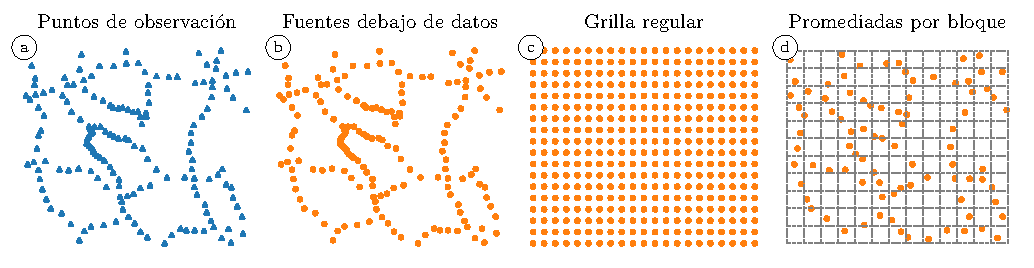
\includegraphics[width=\linewidth]{figs/source-layouts-schematics.pdf}
    \caption{
        Sketch of different horizontal layouts for equivalent source models.
        Blue points represent the locations of observations and orange points
        represent the locations of equivalent sources according to different
        layout strategies.
        (a) Set of \SourceLayoutsSchematicsObservations{} observation points
        that simulate a ground survey.
        (b) Location of the \SourceLayoutsSchematicsSourceBelowData{} sources
        obtained through the \emph{sources-below-data} layout.
        (c) Location of the \SourceLayoutsSchematicsGridSources{} sources
        obtained through the \emph{regular-grid} layout.
        (d) Location of the \SourceLayoutsSchematicsBlockAveragedSources{}
        sources obtained through the \emph{block-averaged sources} layout.
        Grey dashed lines represent the spatial blocks within which the median
        observation location is calculated.
    }
    \label{fig:source_layouts}
\end{figure*}

The most widely used layouts for distributing equivalent sources horizontally
are:

\begin{enumerate}
  \item
    \emph{Sources below data points}: one equivalent source is placed at the
    horizontal location of each data point (Fig.~\ref{fig:source_layouts}b).
    Therefore, the number of sources is be equal to the number of observations
    ($N=M$).
  \item
    \emph{Regular grid}: a homogeneous distribution of point sources below the
    survey region (Fig.~\ref{fig:source_layouts}c). A padding region is often
    added to help reduce edge effects. In practice, it often leads to
    underdetermined problems since a large number of sources is required
    ($N<M$).
\end{enumerate}

For ground surveys, the \emph{regular-grid} layout needs a sufficiently
small grid spacing to be able to fit the observed data.
This creates an unnecessarily large number of sources in areas where no
observations exist.
In contrast, the \emph{sources-below-data} layout is more likely to accurately
fit the observed data with many fewer sources, reducing the computational load.
But when applied to airborne surveys, the \emph{sources-below-data} layout may
place an undesirably large number of sources along the flight paths.
This could lead to aliasing effects on the predicted values, such as the
stripes parallel to flight lines that are often observed when griding airborne
magnetic data.
The \emph{regular-grid} layout can avoid this effect by evenly
distributing sources and using a continuous source layer (e.g.,
right-rectangular prisms or tesseroids).

We propose a new way of distributing equivalent sources horizontally that could
simultaneously reduce the computational load and mitigate some of the drawbacks
of existing layouts.
In the \emph{block-averaged sources} layout,
point sources are placed in the average
position of data points that fall within specified spatial blocks
(Fig.~\ref{fig:source_layouts}d).
This is done by:

\begin{enumerate}
    \item Dividing the survey region into rectangular blocks of equal size.
    \item Computing the median horizontal position of the observation points
      that fall inside each block. Blocks without any observation point are
      omitted.
    \item Assign one point source to the median horizontal position calculated
      in step 1.
\end{enumerate}

The number of sources created by this new layout will be less than the number
of observations if the block size is chosen appropriately (i.e., making sure
that blocks are large enough to contain more than a single data point).
The overdetermined problem that arises from this layout has a lower
computational load and is less prone to overfiting the data since the model
complexity is lower.
Moreover, the block averaging process can balance the spacing between sources
along a flight line and between adjacent lines, helping to reduce aliasing
effects in generated grids.
We will demonstrate through tests on synthetic data that the block-averaged sources
layout is able to interpolate with comparable accuracy to other layouts while
using a fraction of the equivalent sources.


\subsubsection{Depth of sources}

\begin{figure*}
    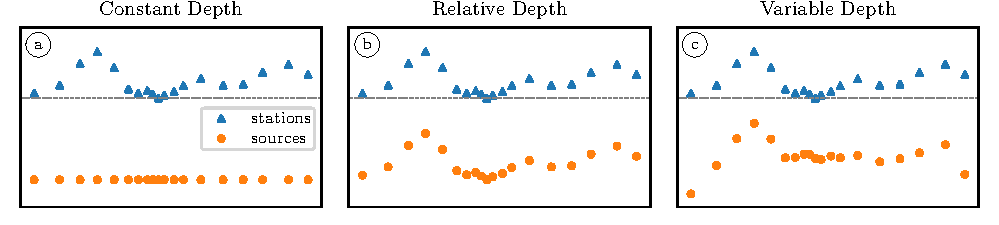
\includegraphics[width=\linewidth]{figs/depth_types.pdf}
    \caption{
        Examples of different strategies for assigning depths to equivalent
        sources.
        Here we assign one source for each
        observation point, located at the same horizontal coordinates as the
        data points.
        Source depths are
        (a)~a \emph{constant depth} at a chosen vertical coordinate,
        (b)~a \emph{relative depth} determined by uniformly shifting the
        vertical coordinate of data points downwards,
        and
        (c)~a \emph{variable depth} determined by shifting the vertical
        coordinates of the observation points by an amount proportional to the
        average distance to neighbouring sources.
        The distance between data points and their respective sources (a)
        depends on observation height, (b) is constant, and (c) is proportional
        to the horizontal distribution of sources.
        Notice how the closely spaced sources in the middle of the profile (c)
        are shallower than their counterparts in (b).
    }
    \label{fig:depth_types}
\end{figure*}

It is widely known from potential theory that the depth of a point source
influences the wavelength of the observed field at the surface.
This makes the source depth a key parameter affecting the outcome of
interpolation and other operations done with equivalent sources.
Several different strategies for assigning the depths of equivalent sources
have been proposed in the literature.
Here, we will highlight the following (Fig.~\ref{fig:depth_types}):

\begin{enumerate}
  \item
    \emph{Constant depth}:
    The simplest option is to locate all sources at the same depth
    (Fig.~\ref{fig:depth_types}a).
    If the measurements were taken at significantly different altitudes, some
    measurements will be more distant to the sources than others,
    which may create problems for reproducing short wavelengths in high
    altitude points.
 \item
    \emph{Relative depth}:
    The depths of sources are determined by shifting the vertical coordinate of
    data points downward by a fixed amount (Fig.~\ref{fig:depth_types}b).
    The sources will not all be at the same vertical coordinate, but they will
    all be at the same vertical distance from the observation points.
 \item
    \emph{Variable depth}:
    The depths of sources are proportional to the horizontal distance to the
    nearest neighbouring data points or sources (Fig.~\ref{fig:depth_types}c).
    Different variations of this strategy have been proposed before, for
    example \citet{cordell1992}, \citet{guspi2004}, and \citet{guspi2009}.
    The rationale for this strategy is that if a survey has data points
    clustered in some areas, we may
    want the sources below those areas to be shallower in order to preserve the
    shorter wavelengths that can be measured.
\end{enumerate}

Our approach to the \emph{variable depth} strategy will be:

\begin{equation}
  z = z_{obs} + \Delta z + \alpha h,
  \label{eq:variable_depth}
\end{equation}

\noindent
in which $z$ is the depth of an equivalent source,
$\Delta z$ is a relative depth shift that is the same for all sources,
$\alpha$ is an adimensional depth factor,
$h$ is the median horizontal distance to the $k$ nearest neighbouring sources,
and
$z_{obs}$ is a vertical observation coordinate that will depend on the
horizontal layout strategy.
For \emph{sources-below-data}, it is the vertical coordinate of the data point
corresponding to the given source.
For \emph{regular-grid}, it can be interpolated from the vertical coordinates
of all data points.
Finally, for \emph{block-averaged-sources} it will be the average vertical
coordinate of data within the corresponding block.

In the following sections, we will test the effectiveness and trade-offs of
each of these strategies on synthetic data.

%%%%%%%%%%%%%%%%%%%%%%%%%%%%%%%%%%%%%%%%%%%%%%%%%%%%%%%%%%%%%%%%%%%%%%%%%%%%%%%

\section{Tests on synthetic data}

\begin{figure*}
    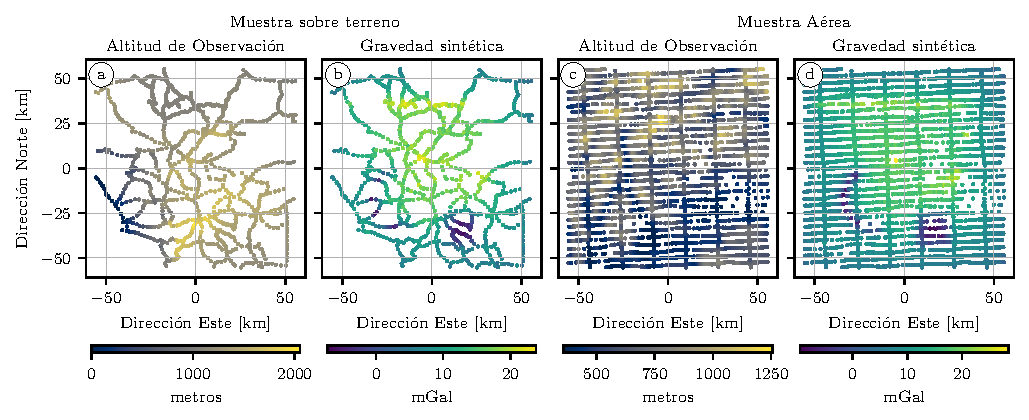
\includegraphics[width=\linewidth]{figs/synthetic-survey-layouts.pdf}
    \caption{
        Maps of the observation locations and gravity values for the synthetic
        ground and airborne surveys.
        (a)~Horizontal position and height of the ground survey points.
        (b)~Synthetic gravity data calculated on the ground survey points with
        added pseudo-random Gaussian noise.
        (c)~Horizontal position and height of the airborne survey points.
        (d)~Synthetic gravity data calculated on the airborne survey points
        with added pseudo-random Gaussian noise.
        Heights are given in meters above the zero height plane.
    }
    \label{fig:synthetic-layouts}
\end{figure*}

\begin{figure}
    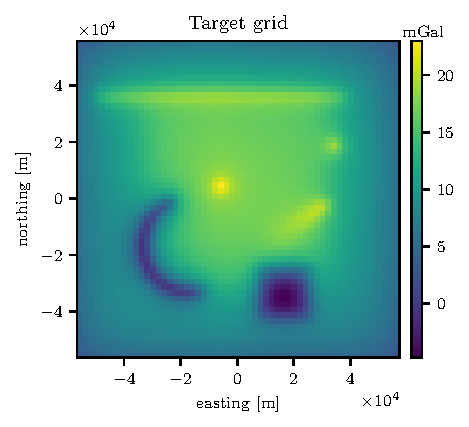
\includegraphics[width=\linewidth]{figs/target-grid.pdf}
    \caption{
        Pseudo-color map of the target grid of synthetic gravity data. The grid
        is composed of \TargetEastingSize{}$\times$\TargetNorthingSize{} points
        with a spacing of \TargetSpacing{}. The grid height is \TargetHeight{}
        above the zero height plane.
    }
    \label{fig:synthetic-target}
\end{figure}

We have used synthetic gravity datasets to test the interpolation accuracy of
the difference horizontal and vertical source distribution strategies as well
as the gradient-boosted equivalent source method.
To generate the data, we created a model that is made out of \NPrisms{}
right-rectangular prisms, distributed on a region of
\ModelEasting{}$\times$\ModelNorthing{} with depths varying between
\ModelDepth{} and zero.
The density contrast of prisms ranges from \ModelMinDensity{} to
\ModelMaxDensity{}.
The model includes prisms of different shapes, sizes, and depths to create
gravity disturbances with a variety of wavelengths.

We created two synthetic datasets from the model, one simulating a ground
survey and another an airborne acquisition (Fig.~\ref{fig:synthetic-layouts}).
To create the synthetic ground survey, we selected measurement positions from a
portion of a public domain dataset for Southern Africa, available through the
NOAA National Centers for Environmental Information (NCEI).
For the synthetic airborne survey, we used a portion of the Great Britain
Aeromagnetic Survey acquired by Hunting Geology and Geophysics Ltd and Canadian
Aeroservices Ltd between 1955 and 1965 and made publicly available by the
British Geological Survey (BGS).
In both cases, we rescaled the horizontal coordinates of each survey portion to
span an area of \SurveyEasting{}$\times$\SurveyNorthing{}, matching the model
dimensions.
The ground survey contains \GroundSurveyPoints{} observations distributed at
heights between \GroundSurveyMinHeight{} and \GroundSurveyMaxHeight{}
(Fig.~\ref{fig:synthetic-layouts}a).
The airborne survey has \AirborneSurveyPoints{} observations at heights between
\AirborneSurveyMinHeight{} and \AirborneSurveyMaxHeight{}.
(Fig.~\ref{fig:synthetic-layouts}c).

The vertical component of the gravitational acceleration generated by the
model was computed  using the method of \citet{nagy2000, nagy2002}
with recent modifications by \citet{fukushima2020},
as implemented in the open-source software Harmonica \citep{harmonica2020}.
We generated a \emph{target grid} of
\TargetEastingSize{}$\times$\TargetNorthingSize{} points with a spacing of
\TargetSpacing{} and located \TargetHeight{} above the zero height plane
(Fig.~\ref{fig:synthetic-target}) to serve as a reference when calculating the
interpolation error.
We then generated synthetic ground (Fig.~\ref{fig:synthetic-layouts}b) and
airborne (Fig.~\ref{fig:synthetic-layouts}d) data to which we added
pseudo-random Gaussian noise with zero mean and \SurveyNoise{} standard
deviation.


\subsection{Source distribution strategies}
\label{sec:synthetic_distributions}

\begin{figure*}
    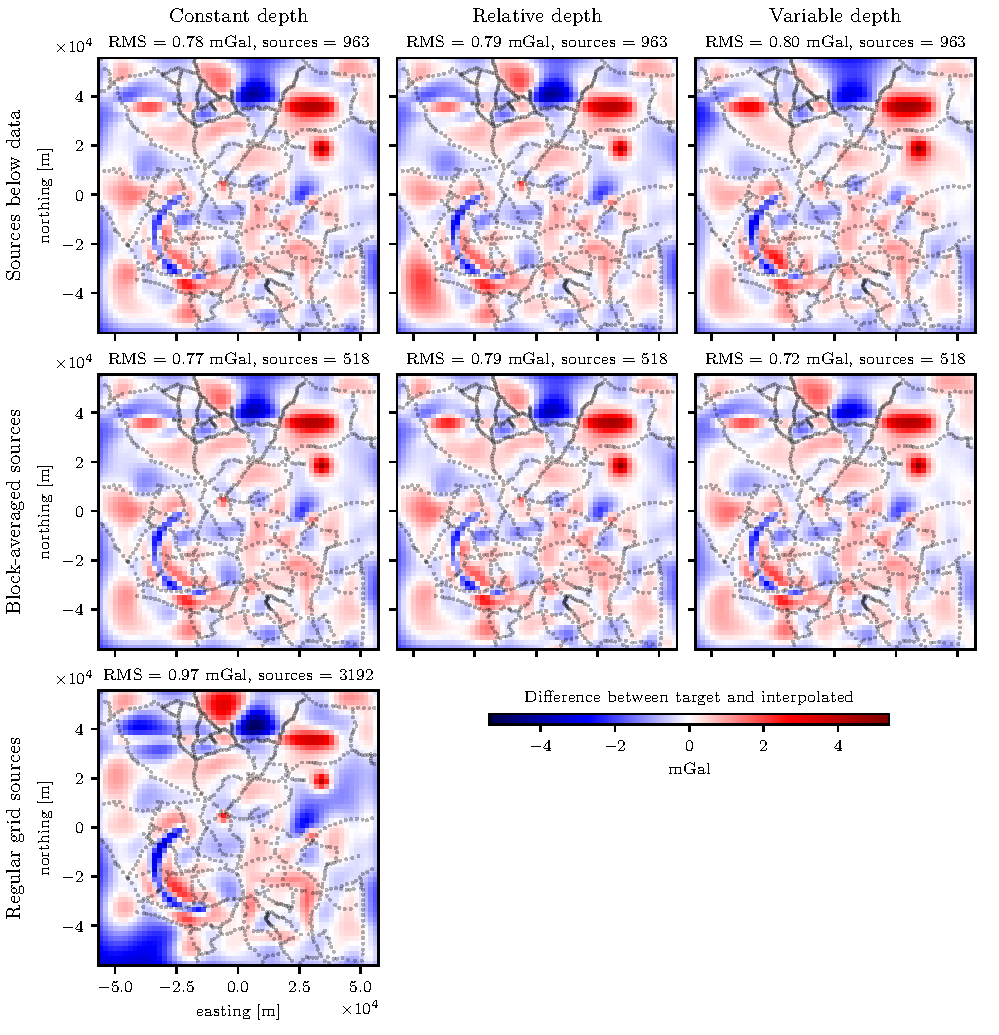
\includegraphics[width=\linewidth]{figs/ground_survey_differences.pdf}
    \caption{
        Pseudo-color maps of the differences between the target grid and the
        interpolated synthetic ground survey data produced by each source
        distribution strategy.
        The black dots represent the horizontal location of the synthetic data
        points. The RMS error and total number of equivalent sources is
        reported for each strategy at the top of the respective maps.
    }
    \label{fig:ground-survey-differences}
\end{figure*}

\begin{figure*}
    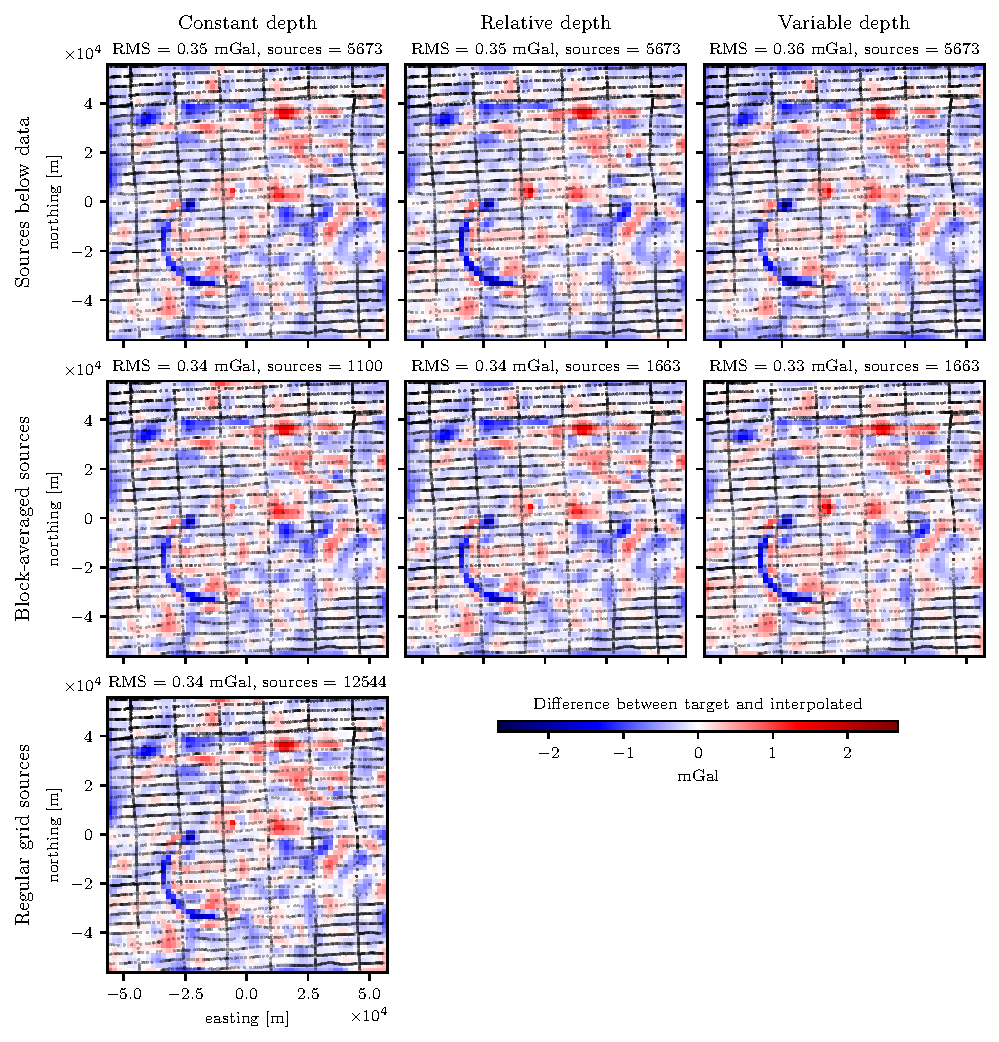
\includegraphics[width=\linewidth]{figs/airborne_survey_differences.pdf}
    \caption{
        Pseudo-color maps of the differences between the target grid and the
        interpolated synthetic airborne survey data produced by each source
        distribution strategy.
        The black dots represent the horizontal location of the synthetic data
        points. The RMS error and total number of equivalent sources is
        reported for each strategy at the top of the respective maps.
    }
    \label{fig:airborne-survey-differences}
\end{figure*}

We investigated the effect of different strategies for distributing the
equivalent sources horizontally and vertically on interpolation accuracy.
To do this, we used the damped least-squares solution described in
Section~\ref{sec:eql_inversion} (without gradient boosting) to interpolate the
synthetic datasets (Fig.~\ref{fig:synthetic-layouts}) and compared the results
against the target grid (Fig.~\ref{fig:synthetic-target}).
This process was repeated for each combination of horizontal layout
(sources-below-data and block-averaged-sources) and depth type (constant,
relative, and variable) and for regular-grid sources with a constant depth,
totalling 7 different combinations.

Each source distribution strategy requires certain hyper-parameters to be
chosen in order to build the set of point sources.
For example, using a constant depth needs the definition of the depth and using
block-average-sources requires the definition of the block size.
The predictive capabilities of the equivalent sources depend on the choice of
these hyper-parameters.
To ensure that our comparisons are fair, we perform an exhaustive search over
combinations of hyper-parameter values (including the damping parameter from
Eq.~\ref{eq:misfit}) to obtain the best prediction that can be achieved by each
source distribution strategy.
Here, the best prediction is defined as the one that minimizes the root
mean-square error (RMS) between interpolated values and the target grid
(Fig.~\ref{fig:synthetic-target}).
The parameter values used in these searches and the one producing the smallest
RMS error are outlined in Tables~\ref{tab:parameters-ground-survey}
and~\ref{tab:parameters-airborne-survey}.

Fig~\ref{fig:ground-survey-differences}
and~\ref{fig:airborne-survey-differences} show the differences between the
target grid and the best prediction achieved by each source distribution
strategy for the ground and airborne synthetic surveys, respectively.
For the synthetic ground survey, the horizontal layouts produced similar RMS
values of approximately \SI{0.8}{\mgal} regardless of the depth type, with the
exception of the regular-grid layout which produced a larger RMS of
\SI{\BestGroundGridSourcesConstantDepthRms{}}{\mgal}.
The differences between the target grid and the interpolated values are larger
in regions of poor data coverage.
Edge effects are present for all strategies but are noticeably smaller for the
combination of block-averaged-sources with a variable depth based on the
nearest neighbour distance.
For the synthetic airborne survey, all strategies (including the regular-grid)
produced similar RMS errors of approximately \SI{0.3}{\mgal}.
The maps of the differences between the target grid and interpolation results
are visually indistinguishable from each other.

%%%%%%%%%%%%%%%%%%%%%%%%%%%%%%%%%%%%%%%%%%%%%%%%%%%%%%%%%%%%%%%%%%%%%%%%%%%%%%%


\subsection{Window size and overlap in gradient boosting}

We assessed the trade-offs in interpolation accuracy and computation time of
the gradient-boosted equivalent sources algorithm as a function of the two key
controlling factors: the window size and the amount of overlap between adjacent
windows.
The comparisons were performed against a regular least-squares solution
(Eq.~\ref{eq:least_squares_solution}) using the synthetic airborne data
(Fig.~\ref{fig:synthetic-layouts}c-d) .
To avoid biasing the results, we used the same locations of equivalent sources
for both the regular and gradient-boosted interpolations, namely
block-averaged-sources with a block size of
\SI{\BestAirborneBlockAveragedSourcesRelativeDepthSpacing}{\meter} and a
relative depth of
\SI{\BestAirborneBlockAveragedSourcesRelativeDepthDepth}{\meter}.

\subsubsection{Window size}
\label{sec:window_size}

The size of the windows controls the size of the Jacobian matrices
$\tilde{\mathbf{A}}_k$ by limiting the number of data points and equivalent
sources used in each step of the gradient-boosting algorithm
(Alg.~\ref{alg:gradient_boosting_window}).
Thus, using smaller windows will reduce the total amount of computer memory
required to estimate the source coefficients.
Nevertheless, smaller windows may produce less accurate interpolations by
failing to achieve the global minimum of the goal function in
Eq.~\ref{eq:misfit}.
The window size might also impact the computation time in non-intuitive ways
since smaller windows generate smaller least-squares problems but also require
more gradient-boosting iterations.

We calculated the interpolation RMS error and computation time for a fixed
window overlap of 50\% and several window sizes.
To avoid any biases introduced by the shuffling of windows, the calculations
were repeated using different seeds for the pseudo-random number generator used
in the shuffling.
Figs.~\ref{fig:gradient-boosted-comparison}a and
\ref{fig:gradient-boosted-comparison}c show the RMS error and computation time
required for estimating the source coefficients, respectively, as a function of
the window size.

The results show that the interpolation RMS error for gradient-boosting is
generally larger than the error for regular equivalent sources.
The error decreases asymptotically to within $\sim 40\%$ of the regular
equivalent sources for windows with an area greater than $\sim 10\%$ of the
survey area.
The computation time similarly decreases with window size, with the
gradient-boosting being generally faster than the regular equivalent sources
for windows with an area greater than $\sim 5\%$ of the survey area.
As the window size increases, both RMS error and computation time appear to
stabilize to nearly constant levels.

\subsubsection{Window overlap}

The amount of overlap between adjacent windows plays an important role in the
performance of the gradient-boosted equivalent sources.
It controls the number of iterations and how often a particular source is used
in the least-squares fitting process.
While the experiments in the previous section showed that 50\% overlap was
sufficient to achieve acceptable interpolation accuracy, we separately studied
the impacts of the amount of window overlap on both accuracy and computation
time.

We performed a similar experiment to one in section~\ref{sec:window_size} but
this time kept the window size fixed to \BoostOverlappingWindowSize{} and
varied the amount of overlap from 0\% to 95\% with a step size of 5\%.
All other experimental procedures remained unchanged.
Figs.~\ref{fig:gradient-boosted-comparison}b and
\ref{fig:gradient-boosted-comparison}d show the RMS error and computation time
required for estimating the source coefficients, respectively, as a function of
the window overlap.

Our results show what the interpolation RMS error decreases with the amount of
overlap, reaching the same accuracy as the regular equivalent sources at
approximately 90\% overlap.
On the other hand, the computation time increases with the amount of overlap,
becoming larger than that of the regular equivalent sources for overlaps
greater than 70\%.
This is expected since increasing the overlap adds iterations to the gradient
boosting algorithm without decreasing the individual least-squares problem
sizes to compensate.

\begin{figure*}
    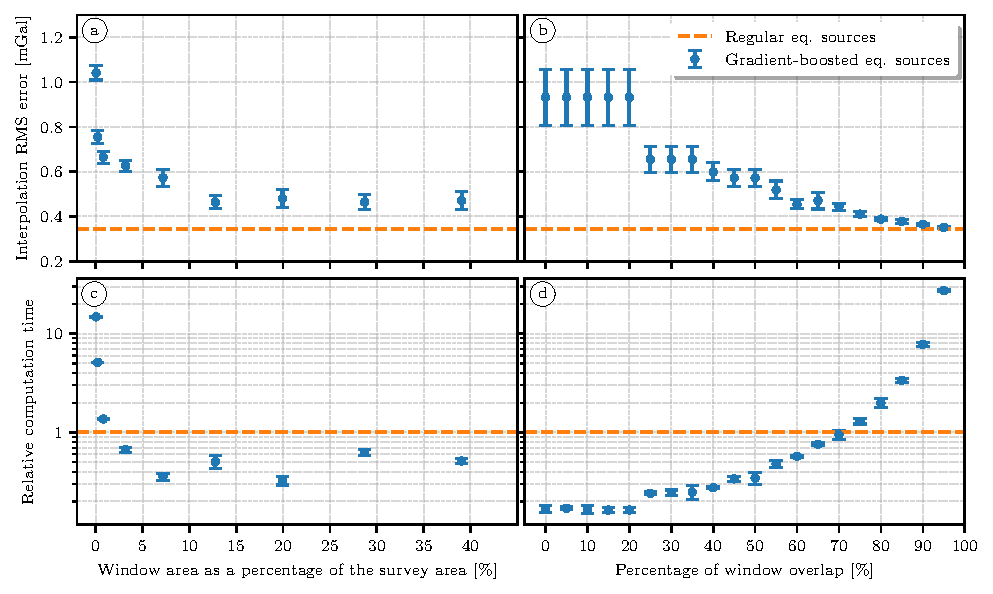
\includegraphics[width=\linewidth]{figs/gradient-boosted-comparisons.pdf}
    \caption{
        Comparison of the interpolation RMS error and computation time for
        regular least-squares equivalent sources (orange dashed lines) and
        gradient-boosted equivalent sources (blue dots and error bars).
        Both methods used the same source positions (block-averaged sources
        with a relative depth).
        Window sizes are given as a percentage of the survey area (e.g., 100\%
        represents a window with the same area as the survey) and window
        overlap is given as a percentage of the window size
        (an overlap of 50\% means that two adjacent windows
        share an area half of the size of the entire window).
        Computation time refers to the time required to estimate the source
        coefficients and is reported as a ratio between the gradient-boosted
        and the regular equivalent sources.
        For gradient-boosting, the RMS errors and computation times are the
        means (error bars represent 1 standard deviation) of results using
        different seeds for the pseudo-random number generator.
        (a)~RMS error between the target grid and interpolation results and
        (b)~computation time as a function of window size.
        (c)~RMS error between the target grid and interpolation results and
        (d)~computation time as a function of window overlap.
}
    \label{fig:gradient-boosted-comparison}
\end{figure*}


%%%%%%%%%%%%%%%%%%%%%%%%%%%%%%%%%%%%%%%%%%%%%%%%%%%%%%%%%%%%%%%%%%%%%%%%%%%%%%%

\section{Gridding gravity data from Australia}

\begin{figure*}
    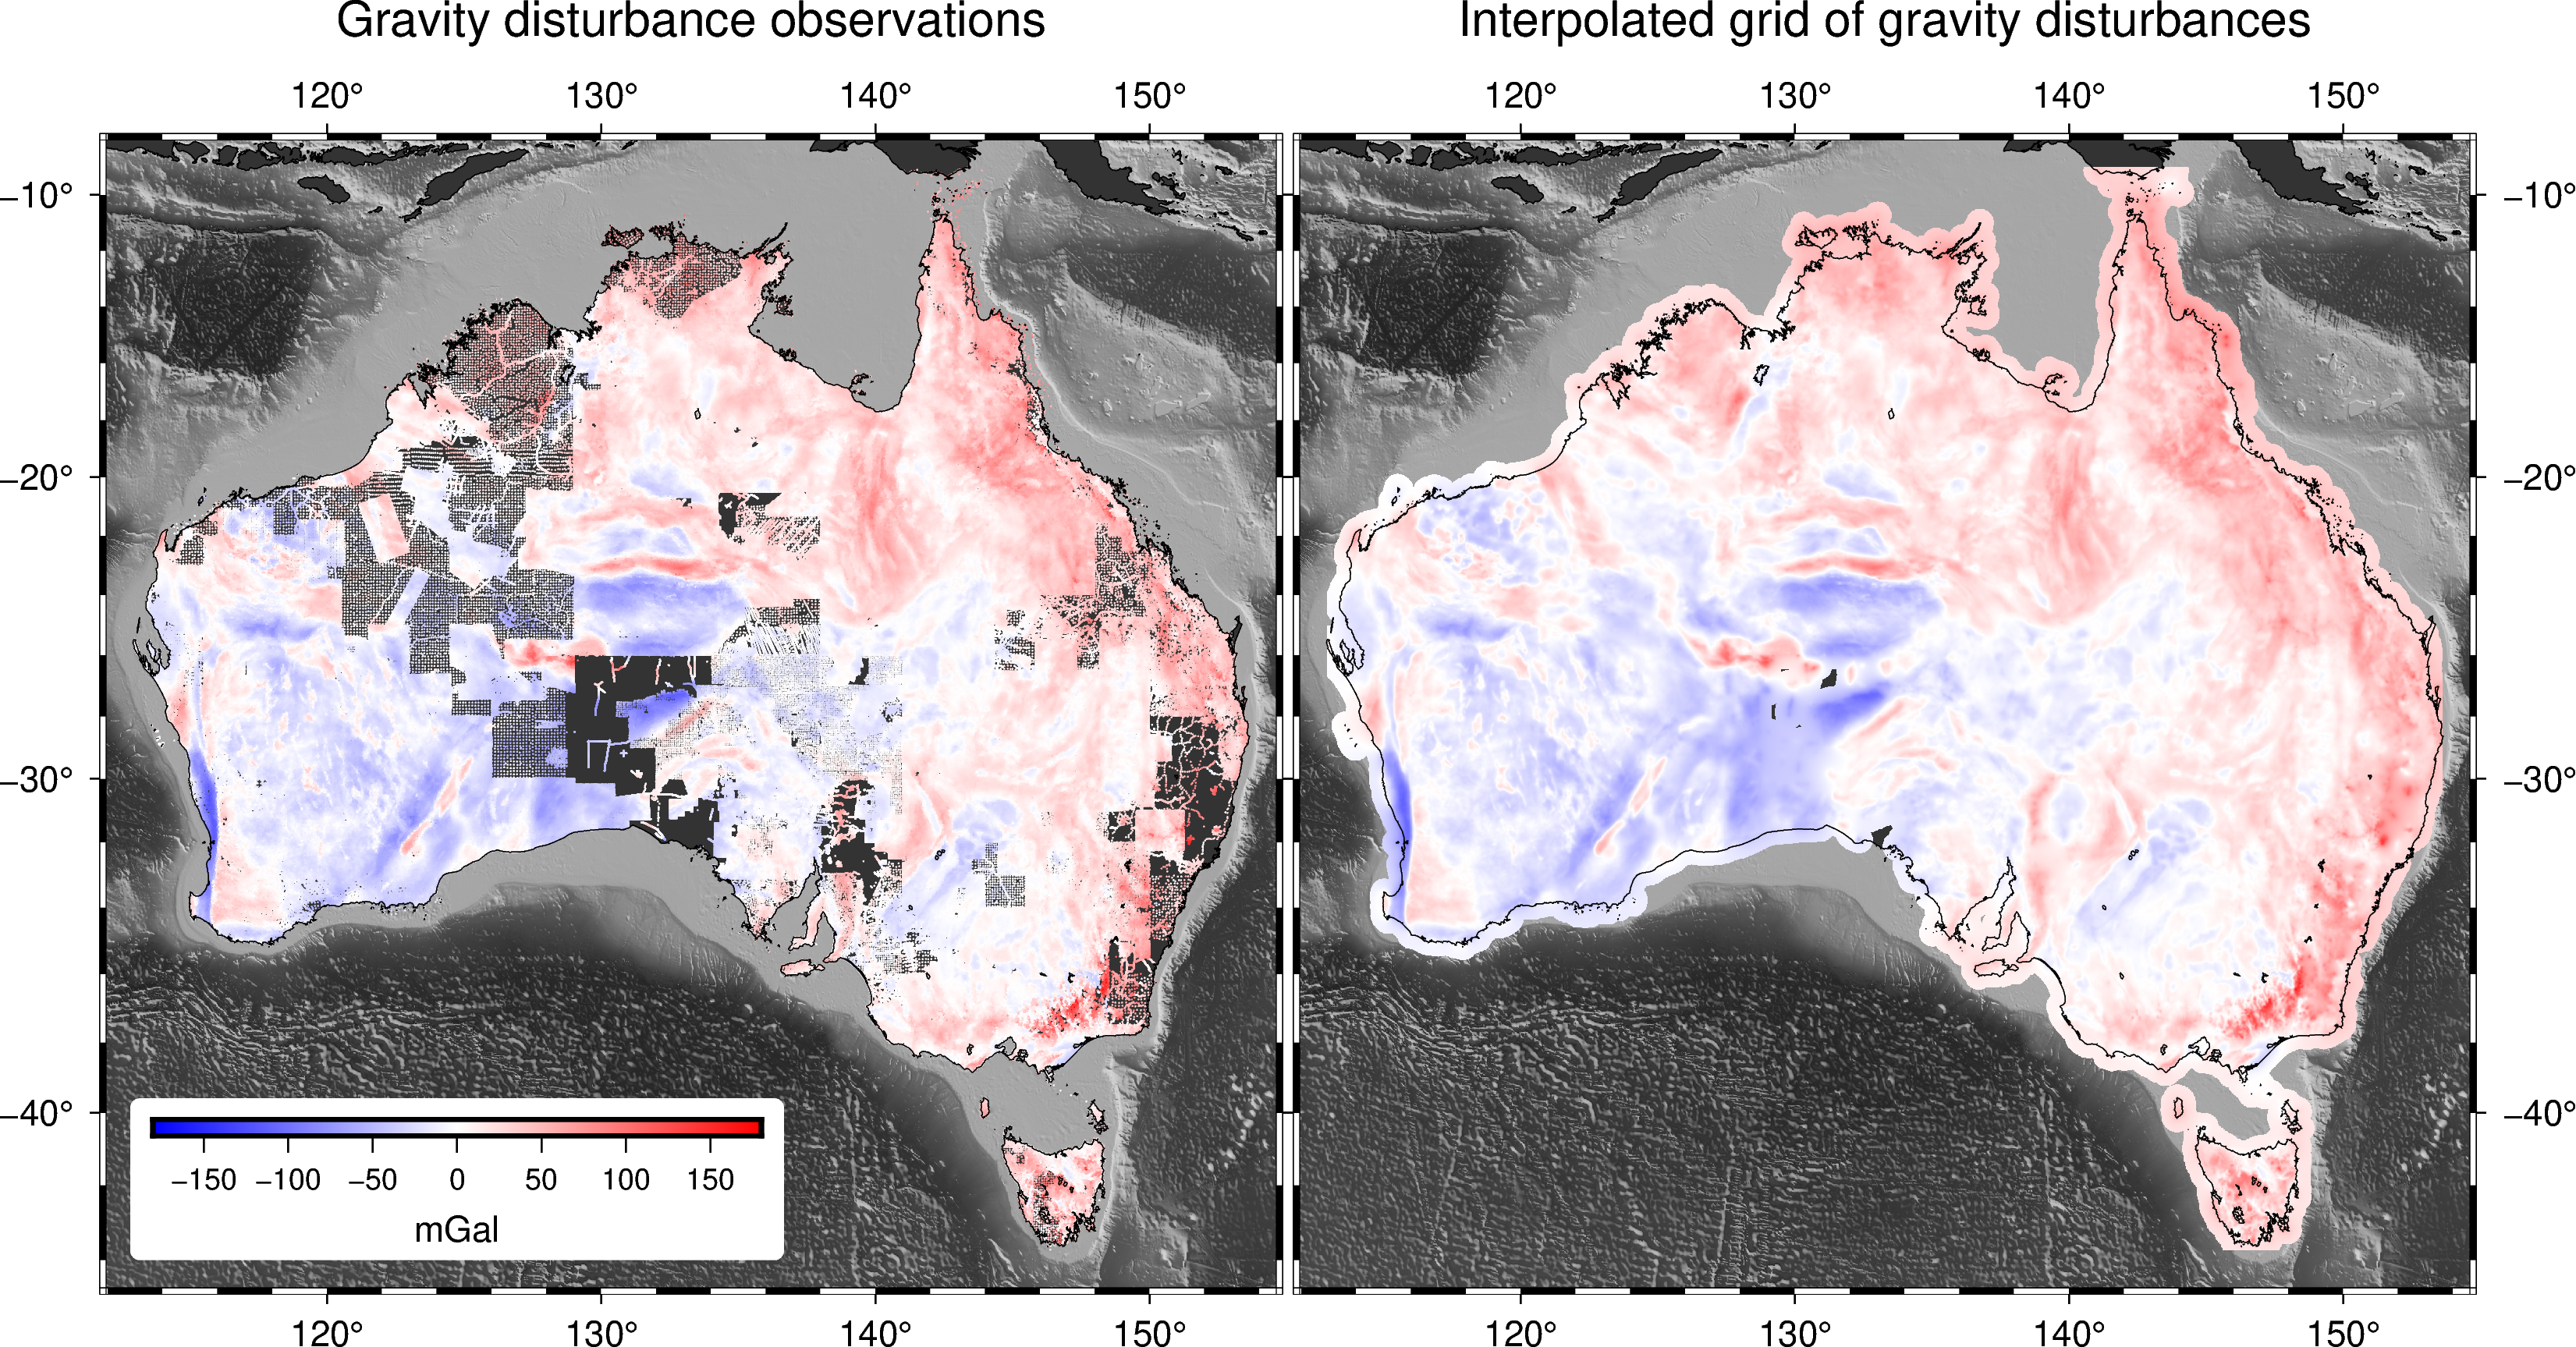
\includegraphics[width=\linewidth]{figs/australia.png}
    \caption{
      Pseudo-color maps of observed (left) and
      interpolated (right) gravity disturbance of Australia.
      Observations are part of a compilation by \citet{wynne2018} of
      over 1.7 million ground gravity measurements.
      Interpolated values were obtained through gradient-boosted equivalent
      sources and calculated on a regular grid at \AustraliaEqlGridHeight{}
      over the WGS84 ellipsoid.
    }
    \label{fig:australia}
\end{figure*}

This section will demonstrate how gradient-boosted equivalent sources can be
used to interpolate large datasets of gravity data onto a regular grid at
uniform height.
For this purpose, we selected an open-access compilation of ground gravity
surveys over Australia made by \citet{wynne2018} and filtered and referenced to
the WGS84 ellipsoid by \citet{australia_compilation}.
It contains over 1.7 million data points and covers most of the Australian
territory at variable point spacings.
Our goal is to create a 1~arc-minute resolution grid of gravity disturbances at
a constant geometric height of \AustraliaEqlGridHeight{} (the largest height of
observations).

We computed the gravity disturbance by removing the normal gravity of
the WGS84 ellipsoid from the observed gravity data (Fig.~\ref{fig:australia}).
Here, normal gravity was computed at each observation point through the
closed-form formula of \citet{ligotze2001} using the Boule software
\citep{boule2020}.
Finally, we converted the observations to planar Cartesian coordinates by
applying a Mercator projection.

We start the interpolation process by defining a set of block-averaged sources
at a relative depth of \AustraliaEqlDepth{} and a block size of
\SI{1.8}{\kilo\meter}, resulting in a total of \AustraliaEqlNSources{}~point
sources.
The block size was chosen to match the desired resolution of the final grid
 (1~arc-minute is approximately \SI{1.8}{\kilo\meter} at the equator).
The coefficients of the gradient-boosted equivalent sources are estimated using
a damping equal to \AustraliaEqlDamping{} and a window size of
\AustraliaEqlWindowSize{}, which was chosen in order to limit the amount of
computer memory needed to store the Jacobian matrix to under 10~Gigabytes.
Finally, we used the estimated source coefficients to predict the values of the
gravity disturbance on a regular grid of
\AustraliaEqlGridNLongitude{}$\times$\AustraliaEqlGridNLatitude{} points at
\AustraliaEqlGridHeight{} above the ellipsoid.
Fig.~\ref{fig:australia} shows the original data distribution and the
interpolated regular grid.
Grid points that are further than \SI{50}{\kilo\meter} from the nearest data
point are masked to avoid unrealistic extrapolations.

The resulting grid preserves the high resolution of the original data while
avoiding aliasing artifacts because to the block averaging.
Some parts of the grid are smoother and with reduced amplitude (e.g., some
southwestern parts), which is expected from the upward continuation that was
performed to have the grid at a constant height.
On a modest workstation with 16 cores and 16~Gigabytes of RAM,
estimating the \AustraliaEqlNSources{} coefficients with gradient-boosting took
$\sim 1.3$~hours and the forward modelling step took $\sim 18$~minutes.

%%%%%%%%%%%%%%%%%%%%%%%%%%%%%%%%%%%%%%%%%%%%%%%%%%%%%%%%%%%%%%%%%%%%%%%%%%%%%%%

\section{Discussion}

\subsection{Location of sources}

The results of our tests on synthetic data
(Figs~\ref{fig:ground-survey-differences}
and~\ref{fig:airborne-survey-differences}) show that there are no significant
differences between source distribution strategies, both in terms of the
interpolation RMS errors and from visual inspection of the difference maps.
Therefore, we argue that all source distribution strategies are able to produce
comparably accurate interpolations.
Nevertheless, the \emph{block-averaged-sources} strategy make use of fewer
sources when compared with other strategies, which reduces the computational
load of estimating the sources coefficients and forward modelling.
To ensure that the interpolation is able to reproduce the high frequencies in
the data, the block size used in the averaging should be chosen to match the
desired grid resolution.

The choice of source depth strategy does not appear to significantly impact the
interpolation RMS error.
In the particular case of a sparse ground survey with block-averaged-sources,
the use of a variable depth visibly reduced edge effects and artifacts in areas
of poor data coverage.
At a first glance, the choice of a depth strategy would not seem to impact
the computation time.
However, when searching for the set of hyper-parameters that produce the most
accurate interpolation (e.g., through cross-validation), one must solve the
inverse problem once for every possible combination of parameters.
A depth strategy like the \emph{variable depth} requires a higher number of
hyper-parameters (depth shift $\Delta z$, depth factor $\alpha$, and the number
of nearest neighbours $k$ from Eq.~\ref{eq:variable_depth}) than other
strategies which only require a single parameter.
Having more parameters means increasing the dimensions of the parameter space
and thus increasing the number of possible combinations.
Thus, we recommend using a \emph{constant depth} or a \emph{relative depth}
when processing large datasets in order to minimize computation time.

\subsection{Gradient boosting}

From Fig.~\ref{fig:gradient-boosted-comparison}a
and~\ref{fig:gradient-boosted-comparison}c, we can see that the
gradient-boosted equivalent sources produce slightly less accurate
interpolation results but are able to achieve smaller computation times than
regular equivalent sources.
The reduction of the accuracy might be due to the gradient boosting algorithm
failing to converge to the global minimum of the goal function.
As the windows increase in size, interpolation error decreases because more data
points are included into the least-squares fitting of the source coefficients.
At the same time, the fitting process becomes faster because of a reduction in
the number of iterations.
Our results indicate that it is desirable to maximize the window size up to the
point that the Jacobian matrices still fit within the available computer
memory.

The results shown in Figs~\ref{fig:gradient-boosted-comparison}b
and~\ref{fig:gradient-boosted-comparison}d indicate that using
window overlap values between 40\% and 70\% strike a balance between
accuracy and computation time.
This corroborates our initial choice of 50\% overlap, which is good enough for
producing accurate predictions in reasonable times.

%%%%%%%%%%%%%%%%%%%%%%%%%%%%%%%%%%%%%%%%%%%%%%%%%%%%%%%%%%%%%%%%%%%%%%%%%%%%%%%

\section{Conclusions}

The equivalent source technique has been proven to be well suited for
interpolating gravity disturbances and magnetic anomalies.
The two main reasons that make it to stand out from other 2D interpolation
methods is the fact that the equivalent sources take into account the height of
the observations and that the interpolated values will always be harmonic
functions.
The main challenge of using equivalent sources in practice is the high
computational load of estimating the coefficients of the equivalent sources,
specially on the computer memory needed to store the Jacobian matrix.
In this work we present two strategies that could be simultaneously applied in
order to interpolate very large datasets (millions of points) in reasonable
computation times on modest hardware:
block-averaging source locations, which reduce the number of equivalent sources
needed for the interpolation,
and the gradient-boosted equivalent source algorithm, which breaks down the
inverse problem into smaller sets of equivalent sources defined by overlapping
windows.
Both methods were tested against synthetic datasets in order to compare their
accuracy and how they perform in terms of computational resources.

Our results show that the block-averaged sources reduce the computational
load needed to estimate source coefficients in comparison to the two traditional
strategies of placing sources below data points or on regular grids.
We also showed that this reduction of the number of sources does not affect
the accuracy of the predictions.
The use of block-averaged sources may also prevent aliasing of the interpolated
values, specially when the observations are unevenly sampled (e.g., airborne
and shipborne surveys).
Special attention must be payed when choosing the size of the blocks for
averaging: as a thumb rule, we recommend choosing a size approximately equal to
the resolution of the regular grid where the values will be interpolated.

Tests that compared strategies for the vertical location of the
sources showed that any one of the three strategies tested
(\emph{constant depth}, \emph{relative depth} and \emph{variable depth})
produces comparable accuracy of interpolation.
Nevertheless, we are more prone to recommending either the \emph{constant
depth} or the \emph{relative depth} for most applications because they involve
less hyper-parameters that would need to be configured before the actual
interpolation.

Gradient-boosted equivalent sources were shown to heavily reduce the computer
memory needed to estimate source coefficients, making it possible to
interpolate large datasets with millions of points that would otherwise produce
Jacobian matrices larger than the available memory.
The interpolations obtained though this new method achieve close to the same
accuracy than the regular equivalent sources (within approximately 40\%), while
reducing the computation time needed to estimate the source coefficients by
approximately three times.
We also show that an overlap of 50\% between adjacent windows achieves a good
compromise between accuracy and computation time.
The size of the overlapping windows should be chosen as the maximum value
possible that creates Jacobian matrices that still fit into computer memory.

The gradient-boosting method developed here can be used in conjunction with any
horizontal source layout, depth strategy, or source type (e.g., point sources,
prisms, tesseroids) because it does not rely on assumptions about the sources.
Future research should investigate the application of gradient boosting to
other equivalent source methods.

%%%%%%%%%%%%%%%%%%%%%%%%%%%%%%%%%%%%%%%%%%%%%%%%%%%%%%%%%%%%%%%%%%%%%%%%%%%%%%%

\section{Data and code availability}

The Python source code used to produce all results and figures presented here
is available at
\url{https://doi.org/10.6084/m9.figshare.13604360} and
\url{https://github.com/compgeolab/eql-gradient-boosted}
under the BSD 3-clause open-source license.

The gradient-boosted equivalent sources implementation is based on the
equivalent source code in the Harmonica library \citep{harmonica2020}.
Other software used in this study includes:
Pooch \citep{pooch2020} for downloading and caching datasets,
Verde \citep{verde2018} for block reductions and coordinate manipulations,
Boule \citep{boule2020} for normal gravity calculations,
xarray \citep{xarray2017} and Numpy \citep{numpy2020} for multidimensional
arrays and numerical computations,
Numba \citep{numba2015} for just-in-time compilation and parallelization,
Matplotlib \citep{matplotlib2007} and PyGMT \citep{pygmt2020} for generating
the figures and maps,
and the Jupyter notebook programming environment \citep{jupyter2016}.
Harmonica, Boule, Pooch, and Verde are part of the Fatiando a Terra project
\citep{fatiando2013}.

All datasets used are open-access and publicly available.
The synthetic surveys were generated using
a public domain gravity dataset for Southern Africa distributed by the
NOAA NCEI (\url{https://www.ngdc.noaa.gov/mgg/gravity/gravity.html})
and the Great Britain Aeromagnetic
Survey distributed by the
British Geological Survey (BGS) under an Open Government License
(\url{https://www.bgs.ac.uk/products/geophysics/aeromagneticRegional.html}).
The shaded relief in Fig.~\ref{fig:australia} is the SRTM15+ dataset by
\citet{tozer2019}.
The Australian ground gravity
data is based on a compilation distributed by Geoscience Australia under a
Creative Commons Attribution 4.0 International Licence \citep{wynne2018}  which
was filtered and referenced to the WGS84 ellipsoid by
\citet{australia_compilation} and is distributed under the same license
(\url{https://doi.org/10.6084/m9.figshare.13643837}).


%%%%%%%%%%%%%%%%%%%%%%%%%%%%%%%%%%%%%%%%%%%%%%%%%%%%%%%%%%%%%%%%%%%%%%%%%%%%%%%

\section{Acknowledgements}

We are indebted to the developers and maintainers of the open-source software
without which this work would not have been possible.
S.R. Soler is supported by a scholarship from CONICET, Argentina.
Contains British Geological Survey materials © UKRI.

S.R. Soler and L. Uieda jointly developed the initial idea, analysed the
results, and wrote the paper. S.R. Soler produced all results and developed the
software implementation with minor revisions by L. Uieda.

%%%%%%%%%%%%%%%%%%%%%%%%%%%%%%%%%%%%%%%%%%%%%%%%%%%%%%%%%%%%%%%%%%%%%%%%%%%%%%%

\bibliographystyle{humannat}
\bibliography{references}

%%%%%%%%%%%%%%%%%%%%%%%%%%%%%%%%%%%%%%%%%%%%%%%%%%%%%%%%%%%%%%%%%%%%%%%%%%%%%%%

\appendix

\section{Source position parameters used for the tests on synthetic data}

Tables~\ref{tab:parameters-ground-survey}
and~\ref{tab:parameters-airborne-survey} show the parameter values tested and
their optimal values for creating the equivalent source distributions tested in
Section~\ref{sec:synthetic_distributions}.
The optimal values were used to produce the results in
Figs~\ref{fig:ground-survey-differences}
and~\ref{fig:airborne-survey-differences}.

\begin{table*}
    \centering
    \caption{
        Parameters used to produce each source distribution for interpolating
        the synthetic ground survey data. Also contains the set of parameters
        that generates the smallest RMS error for each source distribution and
        their corresponding RMS.
    }
    \label{tab:parameters-ground-survey}
    \begin{tabular}{c c l c c c}
        \textbf{Source layout}
            & \textbf{Depth type}
            & \multicolumn{1}{c}{\textbf{Parameters}}
            & \textbf{Values}
            & \textbf{Best}
            & \textbf{RMS} \\
        \toprule

        \multirow{8}{*}{Source Below Data}
            & \multirow{2}{*}{Constant}
                & Depth (m)
                & \GroundSourceBelowDataConstantDepthDepth
                & \BestGroundSourceBelowDataConstantDepthDepth
                & \multirow{2}{*}{
                    \BestGroundSourceBelowDataConstantDepthRms
                  } \\
            &
                & Damping
                & \GroundSourceBelowDataConstantDepthDamping
                & \BestGroundSourceBelowDataConstantDepthDamping
                & \\
            \cmidrule{2-6}
            & \multirow{2}{*}{Relative}
                & Depth (m)
                & \GroundSourceBelowDataRelativeDepthDepth
                & \BestGroundSourceBelowDataRelativeDepthDepth
                & \multirow{2}{*}{
                    \BestGroundSourceBelowDataRelativeDepthRms
                  } \\
            &
                & Damping
                & \GroundSourceBelowDataRelativeDepthDamping
                & \BestGroundSourceBelowDataRelativeDepthDamping
                & \\
            \cmidrule{2-6}
            & \multirow{4}{*}{Variable}
                & Depth (m)
                & \GroundSourceBelowDataVariableDepthDepth
                & \BestGroundSourceBelowDataVariableDepthDepth
                & \multirow{4}{*}{
                    \BestGroundSourceBelowDataVariableDepthRms
                  } \\
            &
                & Depth factor
                & \GroundSourceBelowDataVariableDepthDepthFactor
                & \BestGroundSourceBelowDataVariableDepthDepthFactor
                & \\
            &
                & $k$ neighbours
                & \GroundSourceBelowDataVariableDepthKNearest
                & \BestGroundSourceBelowDataVariableDepthKNearest
                & \\
            &
                & Damping
                & \GroundSourceBelowDataVariableDepthDamping
                & \BestGroundSourceBelowDataVariableDepthDamping
                & \\
        \midrule

        \multirow{11}{*}{Block Averaged Sources}
            & \multirow{3}{*}{Constant}
                & Depth (m)
                & \GroundBlockAveragedSourcesConstantDepthDepth
                & \BestGroundBlockAveragedSourcesConstantDepthDepth
                & \multirow{3}{*}{
                    \BestGroundBlockAveragedSourcesConstantDepthRms
                  } \\
            &
                & Block size (m)
                & \GroundBlockAveragedSourcesConstantDepthSpacing
                & \BestGroundBlockAveragedSourcesConstantDepthSpacing
                & \\
            &
                & Damping
                & \GroundBlockAveragedSourcesConstantDepthDamping
                & \BestGroundBlockAveragedSourcesConstantDepthDamping
                & \\
            \cmidrule{2-6}
            & \multirow{3}{*}{Relative}
                & Depth (m)
                & \GroundBlockAveragedSourcesRelativeDepthDepth
                & \BestGroundBlockAveragedSourcesRelativeDepthDepth
                & \multirow{3}{*}{
                    \BestGroundBlockAveragedSourcesRelativeDepthRms
                  } \\
            &
                & Block size (m)
                & \GroundBlockAveragedSourcesRelativeDepthSpacing
                & \BestGroundBlockAveragedSourcesRelativeDepthSpacing
                & \\
            &
                & Damping
                & \GroundBlockAveragedSourcesRelativeDepthDamping
                & \BestGroundBlockAveragedSourcesRelativeDepthDamping
                & \\
            \cmidrule{2-6}
            & \multirow{5}{*}{Variable}
                & Depth (m)
                & \GroundBlockAveragedSourcesVariableDepthDepth
                & \BestGroundBlockAveragedSourcesVariableDepthDepth
                & \multirow{5}{*}{
                    \BestGroundBlockAveragedSourcesVariableDepthRms
                  } \\
            &
                & Depth factor
                & \GroundBlockAveragedSourcesVariableDepthDepthFactor
                & \BestGroundBlockAveragedSourcesVariableDepthDepthFactor
                & \\
            &
                & $k$ neighbours
                & \GroundBlockAveragedSourcesVariableDepthKNearest
                & \BestGroundBlockAveragedSourcesVariableDepthKNearest
                & \\
            &
                & Block size (m)
                & \GroundBlockAveragedSourcesVariableDepthSpacing
                & \BestGroundBlockAveragedSourcesVariableDepthSpacing
                & \\
            &
                & Damping
                & \GroundBlockAveragedSourcesVariableDepthDamping
                & \BestGroundBlockAveragedSourcesVariableDepthDamping
                & \\
        \midrule

        \multirow{4}{*}{Grid Sources}
            & \multirow{4}{*}{Constant}
                & Depth (m)
                & \GroundGridSourcesConstantDepthDepth
                & \BestGroundGridSourcesConstantDepthDepth
                & \multirow{4}{*}{
                    \BestGroundGridSourcesConstantDepthRms
                  } \\
            &
                & Grid spacing (m)
                & \GroundGridSourcesConstantDepthSpacing
                & \BestGroundGridSourcesConstantDepthSpacing
                & \\
            &
                & Damping
                & \GroundGridSourcesConstantDepthDamping
                & \BestGroundGridSourcesConstantDepthDamping
                & \\
    \end{tabular}
\end{table*}

\begin{table*}
    \centering
    \caption{
        Parameters used to produce each source distribution for interpolating
        the synthetic airborne survey data. Also contains the set of parameters
        that generates the smallest RMS error for each source distribution and
        their corresponding RMS.
    }
    \label{tab:parameters-airborne-survey}
    \begin{tabular}{c c l c c c}
        \textbf{Source layout}
            & \textbf{Depth type}
            & \multicolumn{1}{c}{\textbf{Parameters}}
            & \textbf{Values}
            & \textbf{Best}
            & \textbf{RMS} \\
        \toprule

        \multirow{8}{*}{Source Below Data}
            & \multirow{2}{*}{Constant}
                & Depth (m)
                & \AirborneSourceBelowDataConstantDepthDepth
                & \BestAirborneSourceBelowDataConstantDepthDepth
                & \multirow{2}{*}{
                    \BestAirborneSourceBelowDataConstantDepthRms
                  } \\
            &
                & Damping
                & \AirborneSourceBelowDataConstantDepthDamping
                & \BestAirborneSourceBelowDataConstantDepthDamping
                & \\
            \cmidrule{2-6}
            & \multirow{2}{*}{Relative}
                & Depth (m)
                & \AirborneSourceBelowDataRelativeDepthDepth
                & \BestAirborneSourceBelowDataRelativeDepthDepth
                & \multirow{2}{*}{
                    \BestAirborneSourceBelowDataRelativeDepthRms
                  } \\
            &
                & Damping
                & \AirborneSourceBelowDataRelativeDepthDamping
                & \BestAirborneSourceBelowDataRelativeDepthDamping
                & \\
            \cmidrule{2-6}
            & \multirow{4}{*}{Variable}
                & Depth (m)
                & \AirborneSourceBelowDataVariableDepthDepth
                & \BestAirborneSourceBelowDataVariableDepthDepth
                & \multirow{4}{*}{
                    \BestAirborneSourceBelowDataVariableDepthRms
                  } \\
            &
                & Depth factor
                & \AirborneSourceBelowDataVariableDepthDepthFactor
                & \BestAirborneSourceBelowDataVariableDepthDepthFactor
                & \\
            &
                & $k$ neighbours
                & \AirborneSourceBelowDataVariableDepthKNearest
                & \BestAirborneSourceBelowDataVariableDepthKNearest
                & \\
            &
                & Damping
                & \AirborneSourceBelowDataVariableDepthDamping
                & \BestAirborneSourceBelowDataVariableDepthDamping
                & \\
        \midrule

        \multirow{11}{*}{Block Averaged Sources}
            & \multirow{3}{*}{Constant}
                & Depth (m)
                & \AirborneBlockAveragedSourcesConstantDepthDepth
                & \BestAirborneBlockAveragedSourcesConstantDepthDepth
                & \multirow{3}{*}{
                    \BestAirborneBlockAveragedSourcesConstantDepthRms
                  } \\
            &
                & Block size (m)
                & \AirborneBlockAveragedSourcesConstantDepthSpacing
                & \BestAirborneBlockAveragedSourcesConstantDepthSpacing
                & \\
            &
                & Damping
                & \AirborneBlockAveragedSourcesConstantDepthDamping
                & \BestAirborneBlockAveragedSourcesConstantDepthDamping
                & \\
            \cmidrule{2-6}
            & \multirow{3}{*}{Relative}
                & Depth (m)
                & \AirborneBlockAveragedSourcesRelativeDepthDepth
                & \BestAirborneBlockAveragedSourcesRelativeDepthDepth
                & \multirow{3}{*}{
                    \BestAirborneBlockAveragedSourcesRelativeDepthRms
                  } \\
            &
                & Block size (m)
                & \AirborneBlockAveragedSourcesRelativeDepthSpacing
                & \BestAirborneBlockAveragedSourcesRelativeDepthSpacing
                & \\
            &
                & Damping
                & \AirborneBlockAveragedSourcesRelativeDepthDamping
                & \BestAirborneBlockAveragedSourcesRelativeDepthDamping
                & \\
            \cmidrule{2-6}
            & \multirow{5}{*}{Variable}
                & Depth (m)
                & \AirborneBlockAveragedSourcesVariableDepthDepth
                & \BestAirborneBlockAveragedSourcesVariableDepthDepth
                & \multirow{5}{*}{
                    \BestAirborneBlockAveragedSourcesVariableDepthRms
                  } \\
            &
                & Depth factor
                & \AirborneBlockAveragedSourcesVariableDepthDepthFactor
                & \BestAirborneBlockAveragedSourcesVariableDepthDepthFactor
                & \\
            &
                & $k$ neighbours
                & \AirborneBlockAveragedSourcesVariableDepthKNearest
                & \BestAirborneBlockAveragedSourcesVariableDepthKNearest
                & \\
            &
                & Block size (m)
                & \AirborneBlockAveragedSourcesVariableDepthSpacing
                & \BestAirborneBlockAveragedSourcesVariableDepthSpacing
                & \\
            &
                & Damping
                & \AirborneBlockAveragedSourcesVariableDepthDamping
                & \BestAirborneBlockAveragedSourcesVariableDepthDamping
                & \\
        \midrule

        \multirow{4}{*}{Grid Sources}
            & \multirow{4}{*}{Constant}
                & Depth (m)
                & \AirborneGridSourcesConstantDepthDepth
                & \BestAirborneGridSourcesConstantDepthDepth
                & \multirow{4}{*}{
                    \BestAirborneGridSourcesConstantDepthRms
                  } \\
            &
                & Grid spacing (m)
                & \AirborneGridSourcesConstantDepthSpacing
                & \BestAirborneGridSourcesConstantDepthSpacing
                & \\
            &
                & Damping
                & \AirborneGridSourcesConstantDepthDamping
                & \BestAirborneGridSourcesConstantDepthDamping
                & \\
    \end{tabular}
\end{table*}

\end{document}
